\setchapterpreamble[u]{\margintoc}


\chapter{Input Data Usage}
\labch{input-data-usage}
\index{Input Data Usage}

\marginemptybox{5cm}

In this chapter, we introduce the notion of input data usage as proposed by \sidecite{Urban2018}.
In particular, we include output abstractions in the definition of an unused input variable, obtaining a more general definition.
Through this chapter, we study relations among abstract non-interference and the unused predicate and their use in the context of non-deterministic programs.
Then, we present a \emph{sound and complete} hierarchy of semantics that contains only, and exactly, the information needed to reason about the usage of input variables.
Finally, we show a \emph{sound} abstraction of the unused property collecting syntactic dependencies among variables.
Later in the next chapters, we will define a quantitative measure of usage of input variables, extending the qualitative notion presented in this chapter.


\frenchdiv

\emph{Dans ce chapitre, nous introduisons la notion d'utilisation des données d'entrée telle que proposée par \textcite{Urban2018}. En particulier, nous incluons des abstractions de sortie dans la définition d'une variable d'entrée non utilisée, obtenant ainsi une définition plus générale. Tout au long de ce chapitre, nous étudions les relations entre la non-interférence abstraite et le prédicat de non-utilisation, ainsi que leur utilisation dans le contexte des programmes non déterministes. Ensuite, nous présentons une hiérarchie de sémantiques \emph{correcte et complète} qui contient uniquement, et exactement, les informations nécessaires pour raisonner sur l'utilisation des variables d'entrée. Enfin, nous montrons une abstraction \emph{correcte} de la propriété de non-utilisation en collectant les dépendances syntaxiques entre les variables. Dans les prochains chapitres, nous définirons une mesure quantitative de l'utilisation des variables d'entrée, en étendant la notion qualitative présentée dans ce chapitre.}

\section{Input Data Usage}
\labsec{input-data-usage}

\marginnote{
  The set $\inputvariables$ contains the input variables of the program $\defprogram$, \cf{} \refsec{syntax}.
}
\marginnote{Given a program $\defprogram$, its semantics is defined by the trace semantics $\tracesemantics\in\tracetype$, that is, the set of finite and infinite traces of the program $\defprogram$, \cf{} \refsec{maximal-trace-semantics}.}
\marginnote{Note that, program states $\state$ are tuples of locations $\location$ and values of variables, \cf{} \refsec{syntax}.}
Originally introduced by \textcite{Urban2018}, the notion of input data usage consists in the predicate $\unusedwrapper$ to determine whether the input variables $\definputvariables\in\setof\inputvariables$ are used in the computation of the program's output.
Given the semantics of a program $\defprogram$, the predicate $\unusedwrapper$
holds whenever all the input variables in $\definputvariables$ are not used by the program $\defprogram$.

\marginnote{
  Let $\deftrace\in\finiteinfinitesequences$ be a trace, $\retrieveinput{\deftrace}$ refers to the variable's values of the initial state and $\retrieveoutput{\deftrace}\in\stateandbottom$ to the final ones if $\deftrace$ is of finite length, otherwise $\statebottom$ for non-terminating traces.
}
\marginnote{
  Given a set of variables $\definputvariables\in\setof\inputvariables$, the notation $\retrieveinput{\deftrace}(\definputvariables)\in\valuesofvariables$ refers to the initial values of the variables in $\definputvariables$ in the trace $\deftrace$, where $\valuesofvariables$ is the vector of values for $\cardinalitynospaces{\definputvariables}$ variables.
}
\marginnote{
  From two states $\defstate, \defstate'\in\state$, the notation $\defstate \stateeq{\inputvariableswithoutw} \defstate'$ denotes that the values of the variables in $\inputvariableswithoutw$ are equal in both states, \ie, $\forall \defvariable\in\inputvariableswithoutw$ it holds that $\defstate(\defvariable) = \defstate'(\defvariable)$.
  Locations are not considered in the equality between states.
}
\index{Unused!Predicate}
\begin{definition}[Unused]\labdef{unused-predicate}
  Given a program $\defprogram$ and the set of input variables of interest $\definputvariables\in\setof\inputvariables$, the variables $\definputvariables$ are \emph{unused} if and only if the following predicate holds:
  \begin{eqnarray*}
    \lefteqn{\unusedwrapper(\tracesemantics) \DefifF} \\
    & &\forall
      \defseq\in\tracesemantics, \defvalue\in\valuesofvariables
    .\spacer
      \retrieveinput{\defseq}(\definputvariables) \neq \defvalue \ImplieS \\
      & &\exists
        \defseq'\in\tracesemantics
      .\spacer
        \retrieveinput{\defseq'} \stateeq{\inputvariableswithoutw} \retrieveinput{\defseq}
        \LanD
        \retrieveinput{\defseq'}(\definputvariables) = \defvalue
        \LanD
        \retrieveoutput{\defseq} = \retrieveoutput{\defseq'}
  \end{eqnarray*}
\end{definition}

Intuitively, an input variable $\definputvariable\in \definputvariables$ is unused if all feasible outcomes $\retrieveoutput{\defseq}$ are feasible from all possible initial values of $\definputvariable$.
That is, for all possible initial values $\defvalue$ that differ from the initial value of $\definputvariable$ in the trace $\defseq$, there exists another trace $\defseq'$ with initial value $\defvalue$ for $\definputvariable$ that leads to the same output $\retrieveoutput\defseq$.

\begin{marginlisting}[*-3]
  \caption{Program to check if a student passed the school year.}
  \labprog{school-year}
  \vspace{2\lineheight}
\begin{lstlisting}[style=mystyle,language=Python,escapechar=|]
is_passed(eng, math, sci, plus):
  passing = True;|\labline{initial}|
  if not eng:
    eng = False;|\labline{err1}|
  if not math:
    passing = plus;
  if not math:|\labline{err2}|
    passing = plus;
|\labline{last}|
\end{lstlisting}
\end{marginlisting}

\begin{example}\labexample{school-year}
Let us consider the example program presented in \textcite{Urban2018}, \cf{} \refprog{school-year}.
Based on the boolean-valued input variables \texttt{eng}, \texttt{math}, \texttt{sci}, and \texttt{plus}.
The program should determine whether a student has passed the year or not, and store the result in the variable \texttt{passing}. Additionally, the student is allowed a bonus, \cf{} the variable \texttt{plus}, to help with math and science.
However, there are two mistakes in the program: the statement inside the first conditional should be \texttt{passing = False} (\cf{} \refline{err1}), and the third condition should be \texttt{not sci} instead of \texttt{not math} (\cf{} \refline{err2}).
These two mistakes cause the variables \texttt{eng} and \texttt{sci} to be unused by \refprog{school-year}.
Let us consider the input variable \texttt{sci}.
The trace semantics of the program simplified to consider only the variables \texttt{sci} and \texttt{passing} and omitting intermediate state computations is:
\marginnote[*-5]{
  The notation \[
  \tracetuple{\locinit}{\tuple{\defvalue_1}{\defvalue_2}}\tracearrow\tracetuple{\locend}{\tuple{\defvalue'_1}{\defvalue'_2}}
  \]
  denotes a trace that starts with the state $\tuple{\defvalue_1}{\defvalue_2}$ at the initial location $\locinit$, referring to the initial values of the variables \texttt{sci} and \texttt{passing} respectively, and ends with the final state $\tuple{\defvalue'_1}{\defvalue'_2}$ at the last program location $\locend$. For brevity, we omit the intermediate states of the trace.
}
\begin{align*}
  &{\tracesemanticsnoparam\semanticsof{\texttt{is\_passed}_\texttt{sci}}
  =}\\
  &\quad\left\{
    \begin{array}{l}
      \tracetuple{\locinit}{\tuple{\true}{\anyvalue}}\tracearrow\tracetuple{\loc[9]}{\tuple{\true}{\true}}, \\
      \tracetuple{\locinit}{\tuple{\true}{\anyvalue}}\tracearrow\tracetuple{\loc[9]}{\tuple{\true}{\false}}, \\
      \tracetuple{\locinit}{\tuple{\false}{\anyvalue}}\tracearrow\tracetuple{\loc[9]}{\tuple{\false}{\true}}, \\
      \tracetuple{\locinit}{\tuple{\false}{\anyvalue}}\tracearrow\tracetuple{\loc[9]}{\tuple{\false}{\false}}
    \end{array}
  \right\}
\end{align*}
where the symbol $\anyvalue$ denotes any boolean value, the location $\locinit$ is the initial location (\refline{initial}), and $\loc[9]$ is the last location (\refline{last}).
\reffig{school-year-traces} shows a graphical representation of the trace semantics $\tracesemanticsnoparam\semanticsof{\texttt{is\_passed}_\texttt{sci}}$.
The input variable \texttt{sci} is unused, since each result value for \texttt{passing} is feasible from all possible initial values of \texttt{sci}.

\begin{marginfigure}[*-9]
  \begin{tikzpicture}[scale=0.8]
    \node (linit) at (-0.9,2) {$\locinit:$};
    \node (lend) at (-0.9,0) {$\loc[9]:$};

    % Define the positions of the nodes
    \node (TT) at (0,2) {${\tuple\true\true}$};
    \node (TF) at (1,2) {${\tuple\true\false}$};
    \node (FT) at (2,2) {${\tuple\false\true}$};
    \node (FF) at (3,2) {${\tuple\false\false}$};

    \node (outTT) at (0,0) {${\tuple\true\true}$};
    \node (outTF) at (1,0) {${\tuple\true\false}$};
    \node (outFT) at (2,0) {${\tuple\false\true}$};
    \node (outFF) at (3,0) {${\tuple\false\false}$};

    % Draw the edges
    \draw[->] (TT) -> (outTT);
    \draw[->] (TF) -> (outTT);
    \draw[->] (TT) -> (outTF);
    \draw[->] (TF) -> (outTF);
    \draw[->] (FT) -> (outFT);
    \draw[->] (FF) -> (outFT);
    \draw[->] (FT) -> (outFF);
    \draw[->] (FF) -> (outFF);

    \draw[decorate,decoration={brace,amplitude=8pt,mirror,raise=4pt},yshift=0pt,xshift=-0.1pt] (-1.1,2.2) -- (-1.1,-0.2) node [black,midway,xshift=-0.7cm,rotate=90] {$\tracesemanticsnoparam\semanticsof{\texttt{is\_passed}_\texttt{sci}}$};
\end{tikzpicture}
\caption{Graphical representation of the trace semantics of the \refprog{school-year} considering only the variables \texttt{sci} and \texttt{passing}.}
\labfig{school-year-math-traces}
\end{marginfigure}

Instead, if we consider the variable \texttt{math}, the simplified trace semantics considering only the variables \texttt{math} and \texttt{passing} is:
\begin{align*}
  &{\tracesemanticsnoparam\semanticsof{\texttt{is\_passed}_\texttt{math}}
  =}\\
  &\quad\left\{
    \begin{array}{l}
    \tracetuple{\locinit}{\tuple\true\anyvalue}\tracearrow\tracetuple{\loc[9]}{\tuple\true\true}, \\
    \tracetuple{\locinit}{\tuple\false\anyvalue}\tracearrow\tracetuple{\loc[9]}{\tuple\false\true}, \\
    \tracetuple{\locinit}{\tuple\false\anyvalue}\tracearrow\tracetuple{\loc[9]}{\tuple\false\false}
  \end{array}
  \right\}
\end{align*}
\reffig{school-year-math-traces} shows a graphical representation of the trace semantics $\tracesemanticsnoparam\semanticsof{\texttt{is\_passed}_\texttt{sci}}$.
The input variable \texttt{math} is used, since the result value for \texttt{passing} is not feasible from all possible initial values of \texttt{math}.
Indeed, only the initial value $\tuple\false\anyvalue$ yields the result value $\false$ for \texttt{passing} (in the final state $\tracetuple{\loc[9]}{\tuple\false\false}$).
\end{example}


\begin{marginfigure}[*-11]
  \begin{tikzpicture}[scale=0.8]
    \node (linit) at (-0.9,2) {$\locinit:$};
    \node (lend) at (-0.9,0) {$\loc[9]:$};

    % Define the positions of the nodes
    \node (TT) at (0,2) {${\tuple\true\true}$};
    \node (TF) at (1,2) {${\tuple\true\false}$};
    \node (FT) at (2,2) {${\tuple\false\true}$};
    \node (FF) at (3,2) {${\tuple\false\false}$};

    \node (outTT) at (0,0) {${\tuple\true\true}$};
    \node (outTF) at (1,0) {${\tuple\true\false}$};
    \node (outFT) at (2,0) {${\tuple\false\true}$};
    \node (outFF) at (3,0) {${\tuple\false\false}$};

    % Draw the edges
    \draw[->] (TT) -> (outTT);
    \draw[->] (TF) -> (outTT);
    \draw[->] (FT) -> (outFT);
    \draw[->] (FF) -> (outFT);
    \draw[->] (FT) -> (outFF);
    \draw[->] (FF) -> (outFF);

    \draw[decorate,decoration={brace,amplitude=8pt,mirror,raise=4pt},yshift=0pt,xshift=-0.1pt] (-1.1,2.2) -- (-1.1,-0.2) node [black,midway,xshift=-0.7cm,rotate=90] {$\tracesemanticsnoparam\semanticsof{\texttt{is\_passed}_\texttt{math}}$};
\end{tikzpicture}
\caption{Graphical representation of the trace semantics of the \refprog{school-year} considering only the variables \texttt{math} and \texttt{passing}.}
\labfig{school-year-traces}
\end{marginfigure}

\begin{example}\labexample{syntactic-vs-semantic-usage}
  \begin{marginlisting}
    \caption{Syntactic versus semantic usage of the input variable \texttt{x}.}
    \labprog{syntactic-vs-semantic-usage}
    \vspace{2\lineheight}
  \begin{lstlisting}[style=mystyle,language=Python]
x_plus_rand(x):
  return x + rand();
 \end{lstlisting}
  \end{marginlisting}
With this second example we highlight the difference between the syntactic and semantic meaning of using a variable. Indeed, a variable could be syntactically used in the program, \ie, present in the code, but it could be semantically unused, \ie, it does not affect the computation of the program.
Consider \refprog{syntactic-vs-semantic-usage}, where the input variable \texttt{x} is a non-negative integer.
The variable \texttt{x} is syntactically used by the program, as it is present in the return statement.
However, the variable \texttt{x} is semantically unused if we consider machine integers wrapped up to $\texttt{max\_int}\in\N$.
This difference can be clearly seen by studying the trace semantics of the program. In case of machine integers the trace semantics is, reported also in \reffig{traces-x-plus-rand-max-int}:
\begin{align*}
  &\tracesemanticsnoparam\semanticsof{\texttt{x\_plus\_rand}_{\texttt{max\_int}}}
  =\\
  &\quad\setdef{
    \tracetuple{\locinit}{\langle{x}}\rangle\tracearrow\tracetuple{\loc[3]}{\langle{x+r \mod \texttt{max\_int}}\rangle}
  }{x, r \in \N}
\end{align*}
where $x\in\N$ denotes the value of the input variable \texttt{x} and $r\in\N$ a random integer from the \texttt{rand()} function.
In this case, any outcome value $x+r \mod \texttt{max\_int}$ is feasible from any initial value of \texttt{x}.
Even if $x$ is bigger than a given outcome $z$, the result is still feasible as we can take a positive $r = \texttt{max\_int} - x + z$ to make the wrapped sum $x + r \mod \texttt{max\_int} = z$.
\begin{marginfigure}[*-10]
  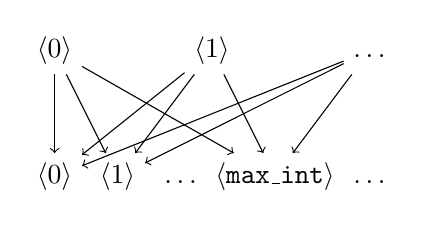
\begin{tikzpicture}[scale=0.8]
    % \node (linit) at (-0.9,2) {$\locinit:$};
    % \node (lend) at (-0.9,0) {$\loc[3]:$};

    % Define the positions of the nodes
    \node (0) at (0,2) {${\langle 0 \rangle}$};
    \node (1) at (2.5,2) {${\langle 1 \rangle}$};
    \node (rest) at (5,2) {\vphantom{${\langle 0 \rangle}$}${\dots}$};

    \node (out0) at (0,0) {${\langle 0 \rangle}$};
    \node (out1) at (1,0) {${\langle 1 \rangle}$};
    \node (outmid) at (2,0) {\vphantom{${\langle 0 \rangle}$}${\dots}$};
    \node (maxint) at (3.5,0) {${\langle \texttt{max\_int} \rangle}$};
    \node (outrest) at (5,0) {\vphantom{${\langle 0 \rangle}$}${\dots}$};

    % Draw the edges
    \draw[->] (0) -> (out0);
    \draw[->] (0) -> (out1);
    % \draw[->] (0) -> (outmid);
    \draw[->] (0) -> (maxint);

    \draw[->] (1) -> (out0);
    \draw[->] (1) -> (out1);
    % \draw[->] (1) -> (outmid);
    \draw[->] (1) -> (maxint);

    \draw[->] (rest) -> (out0);
    \draw[->] (rest) -> (out1);
    % \draw[->] (rest) -> (outmid);
    \draw[->] (rest) -> (maxint);



    % \draw[decorate,decoration={brace,amplitude=8pt,mirror,raise=4pt},yshift=0pt,xshift=-0.1pt] (-1.1,2.2) -- (-1.1,-0.2) node [black,midway,xshift=-0.7cm,rotate=90] {$\tracesemanticsnoparam\semanticsof{\texttt{is\_passed}_\texttt{sci}}$};
\end{tikzpicture}
\caption{Trace semantics of the \refprog{syntactic-vs-semantic-usage} bounded to machine integers.}
\labfig{traces-x-plus-rand-max-int}
\end{marginfigure}

\begin{marginfigure}
  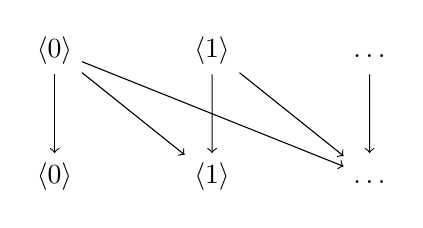
\begin{tikzpicture}[scale=0.8]
    % \node (linit) at (-0.9,2) {$\locinit:$};
    % \node (lend) at (-0.9,0) {$\loc[3]:$};

    % Define the positions of the nodes
    \node (0) at (0,2) {${\langle 0 \rangle}$};
    \node (1) at (2.5,2) {${\langle 1 \rangle}$};
    \node (rest) at (5,2) {\vphantom{${\langle 0 \rangle}$}${\dots}$};

    \node (out0) at (0,0) {${\langle 0 \rangle}$};
    \node (out1) at (2.5,0) {${\langle 1 \rangle}$};
    \node (outrest) at (5,0) {\vphantom{${\langle 0 \rangle}$}${\dots}$};

    % Draw the edges
    \draw[->] (0) -> (out0);
    \draw[->] (0) -> (out1);
    \draw[->] (0) -> (outrest);

    % \draw[->] (1) -> (out0);
    \draw[->] (1) -> (out1);
    \draw[->] (1) -> (outrest);

    % \draw[->] (rest) -> (out0);
    % \draw[->] (rest) -> (out1);
    \draw[->] (rest) -> (outrest);



    % \draw[decorate,decoration={brace,amplitude=8pt,mirror,raise=4pt},yshift=0pt,xshift=-0.1pt] (-1.1,2.2) -- (-1.1,-0.2) node [black,midway,xshift=-0.7cm,rotate=90] {$\tracesemanticsnoparam\semanticsof{\texttt{is\_passed}_\texttt{sci}}$};
\end{tikzpicture}
\caption{Trace semantics of the \refprog{syntactic-vs-semantic-usage}.}
\labfig{traces-x-plus-rand}
\end{marginfigure}
On the other hand, if we consider unbounded positive integers, the trace semantics is:
\begin{align*}
  \tracesemanticsnoparam\semanticsof{\texttt{x\_plus\_rand}_\N}
  =
  \setdef{
    \tracetuple{\locinit}{\langle{x}\rangle}\tracearrow\tracetuple{\loc[3]}{\langle{x+r}\rangle}
  }{x, r \in \N}
\end{align*}
\reffig{traces-x-plus-rand} shows a graphical representation of the trace semantics of the program \refprog{syntactic-vs-semantic-usage} considering unbounded positive integers.
In such instance, for any outcome value $x+r$, only initial values of \texttt{x} that are equal or smaller than $x+r$ may generate such outcome.
For instance, if the outcome is 42, an initial value of 38 is feasible as it exists a random value (\eg, $r = 4$) that makes the sum $38 + 4 = 42$. Instead, an initial value of 43 is not feasible as there is no positive random value $r$ that makes the sum $43 + r = 42$.

In conclusion, the variable \texttt{x} is syntactically used, but it may be semantically unused as it does not affect the computation of the program $\texttt{x\_plus\_rand}_{\texttt{max\_int}}$.
% \pgfplotstableread[]{
% x y
% 0 81
% 1 15
% 2 5
% 3 97
% 4 39
% 5 36
% 6 34
% 7 24
% 8 102
% 9 22
% 10 96
% 11 105
% 12 81
% 13 24
% 14 89
% 15 69
% 16 20
% 17 20
% 18 29
% 19 46
% 20 49
% 21 85
% 22 99
% 23 26
% 24 95
% 25 50
% 26 117
% 27 110
% 28 117
% 29 98
% 30 83
% 31 59
% 32 89
% 33 108
% 34 69
% 35 35
% 36 133
% 37 57
% 38 127
% 39 93
% 40 83
% 41 76
% 42 61
% 43 70
% 44 141
% 45 88
% 46 59
% 47 58
% 48 96
% 49 61
% 50 95
% 51 95
% 52 129
% 53 86
% 54 59
% 55 148
% 56 114
% 57 125
% 58 73
% 59 107
% 60 70
% 61 131
% 62 99
% 63 143
% 64 143
% 65 111
% 66 139
% 67 91
% 68 158
% 69 77
% 70 75
% 71 155
% 72 101
% 73 171
% 74 111
% 75 85
% 76 105
% 77 89
% 78 126
% 79 114
% 80 138
% 81 162
% 82 128
% 83 103
% 84 131
% 85 130
% 86 112
% 87 172
% 88 122
% 89 178
% 90 177
% 91 173
% 92 101
% 93 170
% 94 175
% 95 116
% 96 164
% 97 190
% 98 129
% 99 119
% }\advdata
% \begin{figure}[H]
% \centering
% \caption{Scatterplot of Advertising versus Sales Data}
% \begin{tikzpicture}
% \begin{axis}[
% axis lines = left,
% xlabel = {Input Variable \texttt{x}},
% ylabel = {Program Outcome}
% ]
% \addplot[
% mark=*,only marks,
% point meta =explicit symbolic,
% nodes near coords,
% ]
% table[x=x,y=y]{\advdata};
% \end{axis}
% \end{tikzpicture}
% \end{figure}

\end{example}

\nrefdef{unused-predicate} determines whether a given input variable is used or not, even in the presence of non-deterministic programs%
\sidenote{%
  In \refexample{school-year} the trace semantics where we consider subsets of input variables, \cf{} $\tracesemanticsnoparam\semanticsof{\texttt{is\_passed}_\texttt{sci}}$ and $\tracesemanticsnoparam\semanticsof{\texttt{is\_passed}_\texttt{math}}$, are two non-deterministic sets of traces.
  %
  This can be easily seen by considering the two traces:
  \begin{gather*}
    \tracetuple{\locinit}{\tuple\true\true}\tracearrow\tracetuple{\loc[9]}{\tuple\true\true} \\
       \in \tracesemanticsnoparam\semanticsof{\texttt{is\_passed}_\texttt{sci}} \\
    \tracetuple{\locinit}{\tuple\true\true}\tracearrow\tracetuple{\loc[9]}{\tuple\true\false} \\
       \in \tracesemanticsnoparam\semanticsof{\texttt{is\_passed}_\texttt{sci}}
  \end{gather*}
  where both start from the same initial state $\tuple\true\true$ and have different outcomes.}.
Furthermore, the next example shows that the unused predicate is termination-aware.
Indeed, termination is a possible outcome of a program, and thus a variable should be unused if it does not affect the termination as well as the result of the program.

\begin{marginlisting}
  \caption{Program that does not terminate for positive values of \texttt{x}.}
  \labprog{non-termination}
  \vspace{15pt}
\begin{lstlisting}[style=mystyle,language=Python,escapechar=\%]
non_termination(x):
  while x > 0:
    skip;%\labline{non-terminating-exit}%
  return rand();%\labline{termination-exit}%
 \end{lstlisting}
\end{marginlisting}
\begin{marginfigure}
  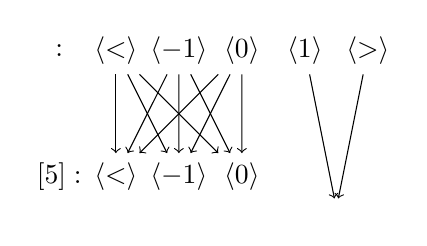
\begin{tikzpicture}[scale=0.8]
    \node (linit) at (-0.9,2) {$\locinit:$};
    \node (lend) at (-0.9,0) {$\loc[5]:$};

    % Define the positions of the nodes
    \node (-2) at (0,2) {${\langle < \rangle}$};
    \node (-1) at (1,2) {${\langle -1 \rangle}$};
    \node (0) at (2,2) {${\langle 0 \rangle}$};
    \node (1) at (3,2) {${\langle 1 \rangle}$};
    \node (2) at (4,2) {${\langle > \rangle}$};

    \node (out-2) at (0,0) {${\langle < \rangle}$};
    \node (out-1) at (1,0) {${\langle -1 \rangle}$};
    \node (out0) at (2,0) {${\langle 0 \rangle}$};
    \node (bot) at (3.5,-0.5) {${\statebottom}$};

    % Draw the edges
    \draw[->] (-2) -> (out-2);
    \draw[->] (-2) -> (out-1);
    \draw[->] (-2) -> (out0);

    \draw[->] (-1) -> (out-2);
    \draw[->] (-1) -> (out-1);
    \draw[->] (-1) -> (out0);

    \draw[->] (0) -> (out0);
    \draw[->] (0) -> (out-1);
    \draw[->] (0) -> (out-2);

    \draw[->] (1) -> (bot);
    \draw[->] (2) -> (bot);
    % \draw[decorate,decoration={brace,amplitude=8pt,mirror,raise=4pt},yshift=0pt,xshift=-0.1pt] (-1.1,2.2) -- (-1.1,-0.2) node [black,midway,xshift=-0.7cm,rotate=90] {$\tracesemanticsnoparam\semanticsof{\texttt{is\_passed}_\texttt{sci}}$};
\end{tikzpicture}
\caption{Trace semantics of the \refprog{non-termination}. The symbol $\statebottom$ denotes non-terminating traces.}
\labfig{traces-non-termination}
\end{marginfigure}
\begin{example}\labexample{non-termination}
  Consider the \refprog{non-termination} defined on the side. The program does not terminate for positive values of \texttt{x} (\cf{} \refline{non-terminating-exit}). Instead, it terminates returning a random value (\cf{} \refline{termination-exit}) if \texttt{x} is negative or equal to $0$. The trace semantics is the following:
  \begin{align*}
    \tracesemanticsnoparam\semanticsof{\texttt{non\_termination}}
    =
    \left\{
    \begin{array}{l}
        \tracetuple{\locinit}{\langle{<}\rangle}\tracearrow\tracetuple{\loc[5]}{\langle{\anyvalue}\rangle}, \\
        \tracetuple{\locinit}{\langle{0}\rangle}\tracearrow\tracetuple{\loc[5]}{\langle{\anyvalue}\rangle}, \\
        \tracetuple{\locinit}{\langle{>}\rangle}\nonterminatingtracearrow\
    \end{array}
    \right\}
  \end{align*}
  where the symbol $<$ denotes a negative value and $>$ a positive one. When the program is provided a positive value for \texttt{x}, it does not terminate and the respective traces are all of infinite length.

  In this example we conclude that the variable \texttt{x} is used since the non-termination is feasible only from positive values of \texttt{x}.
  Otherwise, if we remove non-terminating traces from $\tracesemanticsnoparam\semanticsof{\texttt{non\_termination}}$, the variable \texttt{x} is then unused as it would be totally non-deterministic the outcome of the program.
\end{example}

Note that, the $\unusedwrapper$ predicate (\refdef{unused-predicate}) is equivalent to checking whether each variable separately is unused in the program.

\begin{lemma}\lablemma{single-vs-set-of-variables}
  For all program $\defprogram$ and set of variables $\definputvariables\in\setof\inputvariables$, it holds that:
\[\unusedwrapper(\tracesemantics) \IfF \foralldef{\definputvariable \in \definputvariables}{\unusedwrapperi(\tracesemantics)}
\]
\end{lemma}
\begin{proof}
  Let $\defprogram$ be a program and $\definputvariables\in\setof\inputvariables$ the set of variables of interest.
  To show ($\implies$), we assume that $\unusedwrapper(\tracesemantics)$ holds.
  We need to prove that for all $\definputvariable\in\definputvariables, \deftrace\in\tracesemantics$, and $\defvalue\in\values$ such that $\retrieveinput\deftrace(\definputvariable) \neq \defvalue$, there exists a trace $\deftrace'\in\tracesemantics$ such that $\retrieveinput{\deftrace'}(\definputvariable) = \defvalue$, $\retrieveinput\deftrace \stateeq{\inputvariableswithouti} \retrieveinput{\deftrace'}$, and $\retrieveoutput\deftrace = \retrieveoutput{\deftrace'}$ hold.
  By the definition of $\unusedwrapper(\tracesemantics)$, we have that $\forall \deftrace\in\tracesemantics, \defvalue\in\valuesofvariables.\spacer \retrieveinput{\deftrace}(\definputvariables) \neq \defvalue \implies \exists \deftrace'\in\tracesemantics.\spacer \retrieveinput{\deftrace'} \stateeq{\inputvariableswithoutw} \retrieveinput{\deftrace} \land \retrieveinput{\deftrace'}(\definputvariables) = \defvalue \land \retrieveoutput{\deftrace} = \retrieveoutput{\deftrace'}$. By expanding the definition we obtain:
  \marginnote{
    Given a vector of $n$ values $\defvalue\in\values^n$, we denote the $j$-th value as $\defvalue_j$.
  }
  \begin{align*}
    &\forall \deftrace\in\tracesemantics, \defvalue_1\in\values, \dots, \defvalue_{\cardinalitynospaces{\definputvariables}}\in\values.\\
    &\quad
      \exists j \le \cardinalitynospaces{\definputvariables}.\spacer \retrieveinput{\deftrace}(\definputvariables_j) \neq \defvalue_j \implies \\
    &\quad\quad
      \exists \deftrace'\in\tracesemantics.\spacer
      \forall j \le \cardinalitynospaces{\definputvariables}.\spacer
      \retrieveinput{\deftrace'}(\definputvariables_j) = \defvalue_j \land \\
    &\quad\quad\quad
      \retrieveinput{\deftrace'} \stateeq{\inputvariableswithoutw} \retrieveinput{\deftrace} \land \retrieveoutput{\deftrace} = \retrieveoutput{\deftrace'}
  \end{align*}
  Thus, to prove that it exists a trace $\deftrace'\in\tracesemantics$ such that $\retrieveinput{\deftrace'}(\definputvariable) = \defvalue$, $\retrieveinput\deftrace \stateeq{\inputvariableswithouti} \retrieveinput{\deftrace'}$, and $\retrieveoutput\deftrace = \retrieveoutput{\deftrace'}$ we can take the trace $\deftrace'$ that satisfies the above property where the $j$-th variable of $\definputvariables$ is $\definputvariable$, and we pick the values $\defvalue_1\in\values, \dots, \defvalue_{\cardinalitynospaces{\definputvariables}}\in\values$ such that $\retrieveinput{\deftrace}(\definputvariables_j) \neq \defvalue_j$ but $\retrieveinput{\deftrace}((\definputvariables)_l) = \defvalue_l$ for all the other indices $l$.
  As a consequence, from $\retrieveinput{\deftrace'}(\definputvariables_j) = \defvalue_j \land
    \retrieveinput{\deftrace'} \stateeq{\inputvariableswithoutw} \retrieveinput{\deftrace}$
  it follows that $\retrieveinput{\deftrace'}(\definputvariable) = \defvalue$, $\retrieveinput\deftrace \stateeq{\inputvariableswithouti} \retrieveinput{\deftrace'}$ since all the values of variables in $\definputvariables\setminus{\{\definputvariable\}}$ and $\inputvariableswithoutw$ are equal in both $\deftrace$ and $\deftrace'$.
  Hence, $\deftrace'$ is the trace that satisfies $\unusedwrapperi$, concluding ($\implies$).

  To show ($\Leftarrow$), we assume that $\foralldef{\definputvariable \in \definputvariables}{\unusedwrapperi(\tracesemantics)}$ holds.
  We need to prove that for any trace $\deftrace\in\tracesemantics$ and value $\defvalue\in \valuesofvariables$ such that $\retrieveinput{\deftrace}(\definputvariables) \neq \defvalue$ it exists $\defseq'\in\tracesemantics$ such that $\retrieveinput{\defseq'} \stateeq{\inputvariableswithouti} \retrieveinput{\defseq}$, $
    \retrieveinput{\defseq'}(\definputvariables) = \defvalue$, and $
    \retrieveoutput{\defseq} = \retrieveoutput{\defseq'}$ hold.
  This direction of the implication is less intuitive than the previous one as it requires to show that no changes to multiple variables at the same time can affect the outcome of the program.
  Thus, we focus on values $\defvalue\in\valuesofvariables$ that differ from $\retrieveinput\deftrace(\definputvariables)$ in more than one index, let us call this set of indices that differ as $D\in\setof{\setdef{j\in\N}{j\le\cardinalitynospaces{\definputvariables}}}$. For each $j\in D$, by hypothesis it exists a trace $\defseq^j\in\tracesemantics$ such that $\retrieveinput{\defseq^j} \stateeq{\inputvariables \setminus{\{\definputvariables_j\}}} \retrieveinput{\defseq}$, $
  \retrieveinput{\defseq^j}(\definputvariables_j) = \defvalue_j$, and $
  \retrieveoutput{\defseq} = \retrieveoutput{\defseq^j}$.
  Then, by considering $\defseq^j$ it has to exist another trace $\defseq^{j,l}\in\tracesemantics$ such that $\retrieveinput{\defseq^{j,l}} \stateeq{\inputvariables \setminus{\{\definputvariables_j, (\definputvariables)_l\}}} \retrieveinput{\defseq}$, $
  \retrieveinput{\defseq^{j,l}}(\definputvariables_j, (\definputvariables)_l) = [\defvalue_j\spacer \defvalue_l]$, and $
  \retrieveoutput{\defseq} = \retrieveoutput{\defseq^{j,l}}$ where $l\in D$.
  By repeating this process for all the indices in $D$, we obtain a trace $\defseq'$ that satisfies the property of $\unusedwrapper$. Hence concluding ($\Leftarrow$).
\end{proof}

In the following, we prefer the formalization using sets of variables as originally proposed in \sidetextcite{Urban2018,Urban2020}.

\section{Abstract Input Data Usage}
\labsec{abstract-input-data-usage}

Inspired by the definition of abstract non-interference (ANI) \sidecite{Giacobazzi2018,Mastroeni2023}, reported in \refdef{ani-predicate},
we introduce an abstracted version of the unused predicate.
That is, a version of the unused predicate that abstracts the output states, allowing for a more general definition of the unused property.
Later, we will define the quantitative measure of input data usage, and use the abstraction of output states to determine numerical values from output states.

\index{Abstract Non-Interference}
\marginnote[*-2]{
\begin{definitionshort}[Abstract Non-Interference]\labdef{ani-predicate}
  The abstract non-interference predicate $\aniwrapper$ holds if, for any two traces $\defseq$ and $\defseq'$:
  \begin{gather*}
      \aniselect(\retrieveinput{\defseq}) = \aniselect(\retrieveinput{\defseq'})
      \ImplieS
       \aniobserver(\retrieveoutput{\defseq}) = \aniobserver(\retrieveoutput{\defseq'})
  \end{gather*}
where $\aniselect$ and $\aniobserver$ are upper closure operators on program states to abstract input and output states respectively.
\end{definitionshort}
% We assume that the objective of the input abstraction $\aniselect$ is to monitor the interference of the input variable $\definputvariables$.
}

We define the abstraction of output states, called output observer, as an upper closure operator over states.

\index{Output Observer}
\begin{definition}[Output Observer]\labdef{output-observer}
  Given a program $\defprogram$, an \emph{output observer} $\aniobserver\in \stateandbottom \to \stateandbottom$ is an upper closure operator (\refdef*{upper-closure-operator}[*2.7]) that abstracts the output states.
\end{definition}


We employ the output observer to define an abstract version of the unused predicate, called $\unusediowrapper$, as follows:

\index{Unused!Predicate!Abstract}
\begin{definition}[Abstract Unused]\labdef{abstract-unused}
  Given a program $\defprogram$, an output observer $\aniobserver\in \stateandbottom \to \stateandbottom$, and the input variables of interest $\definputvariables\in\setof\inputvariables$, the variables $\definputvariables$ are (abstractly) \emph{unused} if and only if the following predicate holds:
  \begin{eqnarray*}
    \lefteqn{\unusediowrapper(\tracesemantics) \DefifF} \\
    & &\forall
      \defseq\in\tracesemantics, \defvalue\in\valuesofvariables
    .\spacer
      \retrieveinput{\defseq}(\definputvariables) \neq \defvalue \ImplieS \\
      & &\exists
        \defseq'\in\tracesemantics
      .\spacer
        \retrieveinput{\defseq'} \stateeq{\inputvariableswithouti} \retrieveinput{\defseq}
        \LanD
        \retrieveinput{\defseq'}(\definputvariables) = \defvalue
        \LanD
        \aniobserver(\retrieveoutput{\defseq}) = \aniobserver(\retrieveoutput{\defseq'})
  \end{eqnarray*}
\end{definition}

This abstract unused predicate allows for further abstractions of the output states, which is weaker than the original definition of the unused property.
For instance, the output observer could identify which variable is to consider as the outcome of the program and abstract away the other variables. Another use case could be to abstract the output states into the parity of their variables, or even into the sign. In such case, a variable could be used with respect to \nrefdef{unused-predicate} but unused with respect to \nrefdef{abstract-unused}.

  \begin{marginlisting}[*-2]
    \caption{The variable \texttt{x} is used but not abstractly used.}
    \labprog{parity}
    \vspace{15pt}
  \begin{lstlisting}[style=mystyle,language=Python]
parity(x):
  return 2 * x;
\end{lstlisting}
  \end{marginlisting}
  \begin{example}
  The \refprog{parity} doubles the values of the input variable \texttt{x}. If we consider \nrefdef{unused-predicate}, the variable \texttt{x} is used as for any trace we consider, \eg, the output 4 from an input value of $\texttt{x}=2$, it does not exist a trace that starts with $x > 2$ and terminates with output 4. Instead, by considering the parity of the output value, the \refprog{parity} does not use the variable \texttt{x} as the only possible outcome is ``even.''
\end{example}
  \begin{marginfigure}[*-6]
    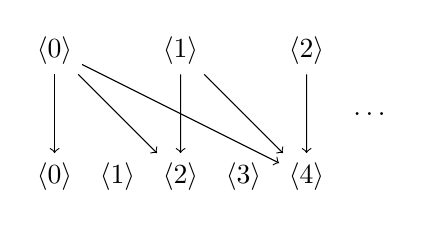
\begin{tikzpicture}[scale=0.8]

      % Define the positions of the nodes
      \node (0) at (0,2) {${\langle 0 \rangle}$};
      \node (1) at (2,2) {${\langle 1 \rangle}$};
      \node (2) at (4,2) {${\langle 2 \rangle}$};

      \node (-) at (5,1) {$\dots$};

      \node (out0) at (0,0) {${\langle 0 \rangle}$};
      \node (out1) at (1,0) {${\langle 1 \rangle}$};
      \node (out2) at (2,0) {${\langle 2 \rangle}$};
      \node (out3) at (3,0) {${\langle 3 \rangle}$};
      \node (out4) at (4,0) {${\langle 4 \rangle}$};

      % Draw the edges
      \draw[->] (0) -> (out0);
      \draw[->] (0) -> (out2);
      \draw[->] (0) -> (out4);

      \draw[->] (1) -> (out2);
      \draw[->] (1) -> (out4);

      \draw[->] (2) -> (out4);
      % \draw[decorate,decoration={brace,amplitude=8pt,mirror,raise=4pt},yshift=0pt,xshift=-0.1pt] (-1.1,2.2) -- (-1.1,-0.2) node [black,midway,xshift=-0.7cm,rotate=90] {$\tracesemanticsnoparam\semanticsof{\texttt{is\_passed}_\texttt{sci}}$};
  \end{tikzpicture}
  \caption{Trace semantics of \refprog{parity} without abstraction.}
  \labfig{parity-without-abstraction}
  \end{marginfigure}
  \begin{marginfigure}[*2]
    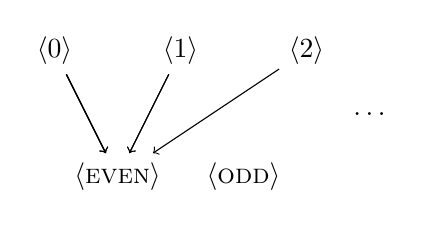
\begin{tikzpicture}[scale=0.8]

      % Define the positions of the nodes
      \node (0) at (0,2) {${\langle 0 \rangle}$};
      \node (1) at (2,2) {${\langle 1 \rangle}$};
      \node (2) at (4,2) {${\langle 2 \rangle}$};

      \node (-) at (5,1) {$\dots$};

      \node (even) at (1,0) {${\langle \textsc{even} \rangle}$};
      \node (odd) at (3,0) {${\langle \textsc{odd} \rangle}$};

      % Draw the edges
      \draw[->] (0) -> (even);
      \draw[->] (0) -> (even);
      \draw[->] (0) -> (even);
      \draw[->] (1) -> (even);
      \draw[->] (1) -> (even);
      \draw[->] (2) -> (even);
      % \draw[decorate,decoration={brace,amplitude=8pt,mirror,raise=4pt},yshift=0pt,xshift=-0.1pt] (-1.1,2.2) -- (-1.1,-0.2) node [black,midway,xshift=-0.7cm,rotate=90] {$\tracesemanticsnoparam\semanticsof{\texttt{is\_passed}_\texttt{sci}}$};
  \end{tikzpicture}
  \caption{Trace semantics of \refprog{parity} with parity abstraction applied to the output states.}
  \labfig{parity}
  \end{marginfigure}

\nrefdef{abstract-unused} can also be seen as a potential abstract non-interference definition working with non-deterministic programs.
As a drawback, we lose the input abstraction: the tread-off allows non-determinism but does not permit input state abstractions in the sense of abstract non-interference.
The reason is that to take into account non-determinism, for any value of the input variables $\definputvariables$, we need to consider all possible traces that start from a different initial value.
Such low-level detail cannot be captured by the input abstraction employed in the definition of abstract non-interference.

The next result shows that the abstract unused predicate is equivalent to the original unused when the output observer is the identity function\sidenote{The identity function returns its parameter without any modification, \ie, $\identity(x) = x$.}.
\index{Unused!Equivalence}
\begin{proposition}[Unused Equivalence]\labprop{unused-predicate-equivalence}
  \marginnote{
    Note that, $\unusedwrapper$ is the unused predicate, \cf{} \nrefdef{unused-predicate}, and $\unusediowrapper$ is the abstract unused predicate, \cf{} \nrefdef{abstract-unused}.
  }
  Whenever $\aniobserver = \identity$, it holds that:
  \begin{gather*}
    \unusedwrapper(\tracesemantics) \IfF \unusediowrapper(\tracesemantics)
  \end{gather*}
\end{proposition}
\begin{proof}
  The proof is straightforward by the definition of the abstract unused predicate, \refdef*{abstract-unused}[*-3.5], and the unused predicate, \refdef*{unused-predicate}[*4.5].
  Indeed, the output observer $\aniobserver = \identity$ does not abstract the output states, and thus the two predicates are equivalent.
\end{proof}

With the use of the next example, we show that non-determinism may affect the abstract non-interference property: non-interfering programs may be wrongly deemed as interfering when non-deterministic statements are present.


\begin{example}\labexample{ani-non-determinism}
  Let us consider the simplified trace semantics of the \refprog{school-year}, considering only the variables \texttt{sci} and \texttt{passing}.
  As this set of traces is non-deterministic, the predicate $\aniwrapper$ would discover that the variable \texttt{sci} interferes with the output states.
  In fact, assuming:
  \marginnote{
    \begin{align*}
      &{\tracesemanticsnoparam\semanticsof{\texttt{is\_passed}_\texttt{sci}}
      =}\\
      &\quad\left\{
        \begin{array}{l}
          \tracetuple{\locinit}{\tuple{\true}{\anyvalue}}\tracearrow\tracetuple{\loc[9]}{\tuple{\true}{\true}}, \\
          \tracetuple{\locinit}{\tuple{\true}{\anyvalue}}\tracearrow\tracetuple{\loc[9]}{\tuple{\true}{\false}}, \\
          \tracetuple{\locinit}{\tuple{\false}{\anyvalue}}\tracearrow\tracetuple{\loc[9]}{\tuple{\false}{\true}}, \\
          \tracetuple{\locinit}{\tuple{\false}{\anyvalue}}\tracearrow\tracetuple{\loc[9]}{\tuple{\false}{\false}}
        \end{array}
      \right\}
    \end{align*}
    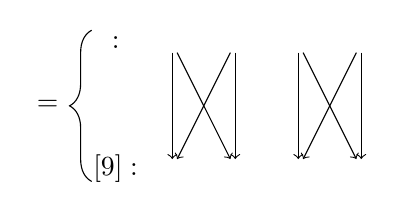
\begin{tikzpicture}[scale=0.8]
      \node (linit) at (-0.9,2) {$\locinit:$};
      \node (lend) at (-0.9,0) {$\loc[9]:$};
      % Define the positions of the nodes
      \node (TT) at (0,2) {${\tuple\true\true}$};
      \node (TF) at (1,2) {${\tuple\true\false}$};
      \node (FT) at (2,2) {${\tuple\false\true}$};
      \node (FF) at (3,2) {${\tuple\false\false}$};
      \node (outTT) at (0,0) {${\tuple\true\true}$};
      \node (outTF) at (1,0) {${\tuple\true\false}$};
      \node (outFT) at (2,0) {${\tuple\false\true}$};
      \node (outFF) at (3,0) {${\tuple\false\false}$};
      % Draw the edges
      \draw[->] (TT) -> (outTT);
      \draw[->] (TF) -> (outTT);
      \draw[->] (TT) -> (outTF);
      \draw[->] (TF) -> (outTF);
      \draw[->] (FT) -> (outFT);
      \draw[->] (FF) -> (outFT);
      \draw[->] (FT) -> (outFF);
      \draw[->] (FF) -> (outFF);
      \draw[decorate,decoration={brace,amplitude=8pt,mirror,raise=4pt},yshift=0pt,xshift=-0.1pt] (-1.1,2.2) -- (-1.1,-0.2) node [black,midway,xshift=-0.7cm] {$=$};
  \end{tikzpicture}
  }
  \begin{align*}
    \eta_{\texttt{sci}}(\defstate) \spacearound{&=} \lambda \texttt{j}. \spacer
    \begin{cases}
      \defstate(\texttt{j}) & \text{if } \texttt{j} \neq \texttt{sci} \\
      \top & \text{otherwise}
    \end{cases}\\
    \aniobserver(\defstate) \spacearound{&=} \defstate
  \end{align*}
  the predicate of  abstract non-interference does not hold for the variable \texttt{sci}.
  This can be shown by the two traces
  \begin{align*}
    \tracetuple{\locinit}{\tuple\true\true}&\tracearrow\tracetuple{\loc[9]}{\tuple\true\true}
    \\
    \tracetuple{\locinit}{\tuple\true\true}&\tracearrow\tracetuple{\loc[9]}{\tuple\true\false}
  \end{align*}
  where the output states are different, but the input states are the same.
  Indeed, $\aniwrapper$ does not take into account that such variation in the outcome may be due to the non-determinism and classifies the variable \texttt{sci} as an interfering variable.
  \end{example}

We formally show that abstract non-interference matches the abstract unused predicate when the program is deterministic, assuming the input abstraction forgets the values of the variables in $\definputvariables$, returning $\top$ otherwise.

\index{Unused!Equivalence}
\begin{proposition}[Abstract Non-Interference Equivalence]\labprop{ani-predicate-equivalence}
  \siderefbox{def}{ani-predicate}
  If $\defprogram$ is deterministic and the input abstraction is defined as:
  \begin{align*}
    \aniselecti(\defstate) \spacearound= \lambda \texttt{j}. \spacer
    \begin{cases}
      \defstate(\texttt{j}) & \text{if } \texttt{j} \not\in \definputvariables \\
      \top & \text{otherwise}
    \end{cases}
  \end{align*}
  then, it holds that:
  \begin{align*}
    \aniwrapper(\tracesemantics) \IfF \unusediowrapper(\tracesemantics)
  \end{align*}
\end{proposition}
\begin{proof}
  % By hypothesis, the program $\defprogram$ is deterministic. Thus, whenever two traces $\deftrace,\deftrace' \in \tracesemantics$ share the same input state, they also share the same output state, \ie, $\retrieveinput\deftrace = \retrieveinput\deftrace' \implies \retrieveoutput\deftrace = \retrieveoutput\deftrace'$.
  To show ($\implies$), we assume $\aniwrapper$.
  Thus, for any two traces $\deftrace, \deftrace'\in\tracesemantics$, it holds that whenever $\aniselecti(\retrieveinput\deftrace) = \aniselecti(\retrieveinput{\deftrace'})$, then $\aniobserver(\retrieveoutput\deftrace) = \aniobserver(\retrieveoutput{\deftrace'})$. By definition of $\aniselecti$, we obtain that the output abstractions match whenever $\retrieveinput\deftrace(\texttt{j}) = \retrieveinput{\deftrace'}(\texttt{j})$ for all variables $\texttt{j} \neq \definputvariables$. This hypothesis can be rewritten as $\retrieveinput\deftrace \stateeq{\inputvariableswithouti} \retrieveinput{\deftrace'}$.
  To prove $\unusediowrapper$,
  let $\deftrace\in\tracesemantics$ be any trace and $\defvalue\in\valuesofvariables$ be any value.
  We assume $\retrieveinput{\deftrace}(\definputvariables) \neq \defvalue$, otherwise the implication is vacuously true.
  We need to show that there exists a trace $\deftrace'\in\tracesemantics$ such that: $(i)$ $\retrieveinput{\deftrace'}(\definputvariables) = \defvalue$, $(ii)$ $\retrieveinput\deftrace \stateeq{\inputvariableswithouti} \retrieveinput{\deftrace'}$, and $(iii)$ $\aniobserver(\retrieveoutput\deftrace) = \aniobserver(\retrieveoutput{\deftrace'})$.
  The proof proceeds by absurd: we assume that for all traces $\deftrace'$ it holds that $\neg(i) \lor \neg(ii) \lor \neg(iii)$.
  By definition of the logical implication\sidenote{$\neg A \lor B \equiv A \implies B$.}, we have that $\neg(\neg(i) \lor \neg(ii)) \implies \neg(iii)$, thus $(i) \land (ii) \implies \neg(iii)$.
  Hence, for all traces $\deftrace'\in\tracesemantics$ we assume $\retrieveinput{\deftrace'}(\definputvariables) = \defvalue$ and $\retrieveinput\deftrace \stateeq{\inputvariableswithouti} \retrieveinput{\deftrace'}$, respectively $(i)$ and $(ii)$.
  As a consequence, to conclude ($\implies$) we need to show an absurd based on the hypothesis that the output abstraction does not match, \ie, $\aniobserver(\retrieveoutput\deftrace) \neq \aniobserver(\retrieveoutput{\deftrace'})$.
  Clearly, from $\aniwrapper$ applied to $(ii)$ we have that the outputs match, contradicting the hypothesis. Thus, $\unusediowrapper$ holds\sidenote{
  Note that, to show ($\implies$) we do not need the assumption that $\defprogram$ is deterministic.}.

  To show ($\Leftarrow$), we assume $\unusediowrapper$.
  For any trace $\deftrace\in\tracesemantics$ and value $\defvalue\in\valuesofvariables$, it holds that whenever $(a)$ $\retrieveinput{\deftrace}(\definputvariables) \neq \defvalue$, then it exists a trace $\deftrace'\in\tracesemantics$ such that $(b)$ $\retrieveinput{\deftrace'}(\definputvariables) = \defvalue$, $(c)$ $\retrieveinput\deftrace \stateeq{\inputvariableswithouti} \retrieveinput{\deftrace'}$, and $(d)$ $\aniobserver(\retrieveoutput\deftrace) = \aniobserver(\retrieveoutput{\deftrace'})$ hold.
  To prove $\aniwrapper$, we assume that for any two traces $\deftrace, \deftrace'\in\tracesemantics$ it holds that $\retrieveinput{\deftrace} \stateeq{\inputvariableswithouti} \retrieveinput{\deftrace'}$, otherwise $\aniwrapper$ vacuously holds. We need to show that the output abstraction of the two traces match, \ie, $\aniobserver(\retrieveoutput\deftrace) = \aniobserver(\retrieveoutput{\deftrace'})$.
  Let $\defvalue\in\valuesofvariables$ be any value.
  \begin{enumerate}
    \item If $\retrieveinput{\deftrace}(\definputvariables) = \retrieveinput{\deftrace'}(\definputvariables) = \defvalue$, then by determinism of $\defprogram$ it follows that $(d)$, \cf{} $\retrieveoutput\deftrace = \retrieveoutput{\deftrace'}$, must hold.
    \item If $\retrieveinput{\deftrace}(\definputvariables) \neq \retrieveinput{\deftrace'}(\definputvariables)$, we let $\retrieveinput{\deftrace}(\definputvariables) \neq \defvalue$ and $\retrieveinput{\deftrace'}(\definputvariables) = \defvalue$ without loss of generality, respectively proving $(a)$ and $(c)$. $(b)$ holds by hypothesis. Hence, from $\unusediowrapper$ it follows that $(d)$ must hold:
    \begin{align*}
      &\forall \deftrace\in\tracesemantics, \defvalue\in\valuesofvariables.\spacer \\
      &\quad (a) \implies \exists \deftrace'\in\tracesemantics.\spacer (b) \land (c) \land (d) && \iff \\
      &\quad \neg(a) \lor (\exists \deftrace'\in\tracesemantics.\spacer (b) \land (c) \land (d)) && \iff \\
      &\quad (\exists \deftrace'\in\tracesemantics.\spacer (b) \land (c) \land (d)) \lor \neg(a) && \iff \\
      &\quad  \neg(\exists \deftrace'\in\tracesemantics.\spacer (b) \land (c) \land (d)) \implies \neg(a) && \iff \\
      &\quad  (\forall \deftrace'\in\tracesemantics.\spacer \neg(b) \lor \neg(c) \lor \neg(d)) \implies \neg(a) && \iff \\
      &\quad  (\forall \deftrace'\in\tracesemantics.\spacer \neg(\neg(b) \lor \neg(c)) \implies \neg(d)) \implies \neg(a) && \iff \\
      &\quad  (\forall \deftrace'\in\tracesemantics.\spacer (b) \land (c) \implies \neg(d)) \implies \neg(a)
    \end{align*}
    Thus, everything resolves around whether $(d)$ holds or not.
    If $(d)$ does not hold, then $\neg(a)$ holds, but this contradicts the hypothesis that $(a)$ holds, hence $(d)$ must hold and so $\aniwrapper$.
    Otherwise, if $(d)$ holds, then $\aniwrapper$ holds.
    Concluding ($\Leftarrow$).
  \end{enumerate}
  % In such case, we also take into consideration that $\defprogram$ is deterministic.
  % Thus, whenever two traces $\deftrace,\deftrace' \in \tracesemantics$ share the same input state, they also share the same output state, \ie, $\retrieveinput\deftrace = \retrieveinput\deftrace' \implies \retrieveoutput\deftrace = \retrieveoutput\deftrace'$.
  % Let us fix the trace $\deftrace\in\tracesemantics$ and value $\defvalue\in\valuesofvariables$, either we assume that $\retrieveinput{\deftrace}(\definputvariables) \neq \defvalue$ \ref{ani-predicate-equivalence-0} or $\retrieveinput{\deftrace}(\definputvariables) = \defvalue$ \ref{ani-predicate-equivalence-1} holds.
  % \begin{enumerate}[label=(\roman*)]
  %   \item \label{ani-predicate-equivalence-0} In case we assume $\retrieveinput{\deftrace}(\definputvariables) \neq \defvalue$, then by $\unusediowrapper$ it exists a trace $\deftrace'\in\tracesemantics$ such that $\retrieveinput{\deftrace'}(\definputvariables) = \defvalue$, $\retrieveinput\deftrace \stateeq{\inputvariableswithouti} \retrieveinput{\deftrace'}$, and $\aniobserver(\retrieveoutput\deftrace) = \aniobserver(\retrieveoutput{\deftrace'})$ hold. By assumption of $\aniwrapper$, for all two traces $\retrieveinput\deftrace \stateeq{\inputvariableswithouti} \retrieveinput{\deftrace'}$ holds, hence we need to show that any trace $\deftrace'\in\tracesemantics$ share the same output abstraction as $\deftrace$. It is easy to see that if $\retrieveinput{\deftrace'}(\definputvariables) = \defvalue$ by $\unusediowrapper$ then they also share the same output abstraction.
  %   \item \label{ani-predicate-equivalence-1} On the other hand, we assume that $\retrieveinput{\deftrace}(\definputvariables) \neq \defvalue$, hence $\unusediowrapper$ cannot prove our conclusion when applied to $\deftrace$ and $\defvalue$. However, either it exists a value $\defvalue'\in\valuesofvariables$ such that $\defvalue \neq \defvalue'$ or $\valuesofvariables=\{\defvalue\}$. In the latter, $\aniwrapper$ holds from the fact that any variable only input value is $\defvalue$ and the program $\defprogram$ is deterministic, thus $\tracesemantics$ contains only a single trace. Otherwise, we apply $\unusediowrapper$ to $\deftrace$ and the value $\defvalue'$.
  %   From here, it follows the same conclusion of the previous point \ref{ani-predicate-equivalence-0}
  % \end{enumerate}
\end{proof}

\begin{example}\labexample{determinization}
  Interestingly, with the use of ``seeds'' one could also determinize a non-deterministic semantics by fixing the random observations as part of the program states.
  Consider the set of traces of the previous example, \cf{} $\tracesemanticsnoparam\semanticsof{\texttt{is\_passed}_\texttt{sci}}$, but with the addition of a random variable that is used to determinize the outcome of the program.
  A possible determinization could be the set of traces:
  \marginnote[*-1]{
    \begin{align*}
      &{\tracesemanticsnoparam\semanticsof{\texttt{is\_passed}_\texttt{sci}}
      =}\\
      &\quad\left\{
        \begin{array}{l}
          \tracetuple{\locinit}{\tuple{\true}{\anyvalue}}\tracearrow\tracetuple{\loc[9]}{\tuple{\true}{\true}}, \\
          \tracetuple{\locinit}{\tuple{\true}{\anyvalue}}\tracearrow\tracetuple{\loc[9]}{\tuple{\true}{\false}}, \\
          \tracetuple{\locinit}{\tuple{\false}{\anyvalue}}\tracearrow\tracetuple{\loc[9]}{\tuple{\false}{\true}}, \\
          \tracetuple{\locinit}{\tuple{\false}{\anyvalue}}\tracearrow\tracetuple{\loc[9]}{\tuple{\false}{\false}}
        \end{array}
      \right\}
    \end{align*}
  }
  \begin{marginfigure}[*5]
    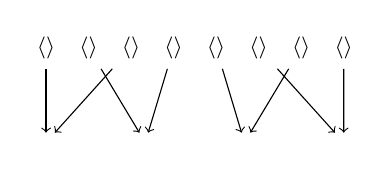
\begin{tikzpicture}[scale=0.6]
      \def\step{0.9}
      % Define the positions of the nodes
      \node (TTT) at (0,2) {\footnotesize${\langle\true\true\true\rangle}$};
      \node (TTF) at (1*\step,2) {\footnotesize${\langle\true\true\false\rangle}$};
      \node (TFT) at (2*\step,2) {\footnotesize${\langle\true\false\true\rangle}$};
      \node (TFF) at (3*\step,2) {\footnotesize${\langle\true\false\false\rangle}$};
      \node (FTT) at (4*\step,2) {\footnotesize${\langle\false\true\true\rangle}$};
      \node (FTF) at (5*\step,2) {\footnotesize${\langle\false\true\false\rangle}$};
      \node (FFT) at (6*\step,2) {\footnotesize${\langle\false\false\true\rangle}$};
      \node (FFF) at (7*\step,2) {\footnotesize${\langle\false\false\false\rangle}$};
      \node (TT) at (0,0) {$\tuple\true\true$};
      \node (TF) at (2.1,0) {$\tuple\true\false$};
      \node (FT) at (4.2,0) {$\tuple\false\true$};
      \node (FF) at (7*\step,0) {$\tuple\false\false$};
      % Draw the edges
      \draw[->] (TTT) -> (TT);
      \draw[->] (TTF) -> (TF);
      \draw[->] (TFT) -> (TT);
      \draw[->] (TFF) -> (TF);
      \draw[->] (FTT) -> (FT);
      \draw[->] (FTF) -> (FF);
      \draw[->] (FFT) -> (FT);
      \draw[->] (FFF) -> (FF);
      % \draw[decorate,decoration={brace,amplitude=8pt,mirror,raise=4pt},yshift=0pt,xshift=-0.1pt] (-1.1,2.2) -- (-1.1,-0.2) node [black,midway,xshift=-0.7cm] {$=$};
  \end{tikzpicture}
  \caption{Trace semantics of \refprog{school-year} with determinization (third component of initial states).}
  \labfig{determinized}
\end{marginfigure}
  \begin{eqnarray*}
    \left\{
      \begin{array}{l}
        \tracetuple{\locinit}{\langle{\true,\true,\true}\rangle}\tracearrow\tracetuple{\loc[9]}{\tuple\true\true}, \\
        \tracetuple{\locinit}{\langle{\true,\true,\false}\rangle}\tracearrow\tracetuple{\loc[9]}{\tuple\true\false}, \\
        \tracetuple{\locinit}{\langle{\true,\false,\true}\rangle}\tracearrow\tracetuple{\loc[9]}{\tuple\true\true}, \\
        \tracetuple{\locinit}{\langle{\true,\false,\false}\rangle}\tracearrow\tracetuple{\loc[9]}{\tuple\true\false}, \\
        \tracetuple{\locinit}{\langle{\false,\true,\true}\rangle}\tracearrow\tracetuple{\loc[9]}{\tuple\false\true}, \\
        \tracetuple{\locinit}{\langle{\false,\true,\false}\rangle}\tracearrow\tracetuple{\loc[9]}{\tuple\false\false} \\
        \tracetuple{\locinit}{\langle{\false,\false,\false}\rangle}\tracearrow\tracetuple{\loc[9]}{\tuple\false\true}, \\
        \tracetuple{\locinit}{\langle{\false,\false,\false}\rangle}\tracearrow\tracetuple{\loc[9]}{\tuple\false\false}
      \end{array}
    \right\}
  \end{eqnarray*}
  where the last component of input states is the boolean seed used to determine the outcome of the program.
  \reffig{determinized} shows the traces in a graphical representation.
  In such instance, the semantics is deterministic as it is not possible anymore to have two traces with the same input states and different output states.
  Thus, the predicate $\aniwrapper$ and $\unusediowrapper$ are equivalent in such instance.
\end{example}

Combining both non-interference and input data usage into the abstract notion of $\unusediowrapper$ permits instances of abstract non-interference to work in the context of non-deterministic programs.
For example, the \emph{non-exploitability} property \sidecite{Parolini2024} is an instance of abstract non-interference where the output states are abstracted to a flag that indicates whether the program reached an error state or not.
Specifically, the state maps the error flag (called \neerror{} in \refdef{ne-predicate}) to a value indicating whether an error state has been reached during the execution or not.
The non-exploitability property holds if, for any variation of the variables $\definputvariables\in\setof\inputvariables$, the program does not reach an error state (or it does so consistently across all the traces). The idea is to prove that an attacker is not able to exploit an error state based on the values of public variables under their control.
When such property is plugged into $\unusediowrapper$, it convenes a non-exploitability definition for non-deterministic programs.


\marginnote[*-2]{
\begin{definitionshort}[Non-Exploitability]\labdef{ne-predicate}
  Let $\definputvariables\in\setof\inputvariables$ be the set of public input variables.
  The \emph{non-exploitability} predicate $\newrapper$ holds if, for any two traces $\defseq$ and $\defseq'$:
  \begin{align*}
      &\retrieveinput{\defseq} \stateeq{\inputvariableswithoutw} \retrieveinput{\defseq'}
      \ImplieS \\
      &\quad \retrieveoutput{\defseq}(\neerror) = \retrieveoutput{\defseq'}(\neerror)
  \end{align*}
\end{definitionshort}
}

\index{Non-Exploitability}
\begin{definition}[Non-Exploitability for Non-Deterministic Programs]\labdef{ne-unused}
  Let $\definputvariables\in\setof\inputvariables$ be the set of public input variables.
  The \emph{non-exploitability predicate for non-deterministic programs} is defined as follows:
  \begin{align*}
    &\newrapper(\tracesemantics) \DefifF \\
    &\quad\forall
      \defseq\in\tracesemantics, \defvalue\in\valuesofvariables
    .\spacer
      \retrieveinput{\defseq}(\definputvariables) \neq \defvalue \ImplieS \\
      &\quad\exists
        \defseq'\in\tracesemantics
      .\spacer
        \retrieveinput{\defseq'} \stateeq{\inputvariableswithouti} \retrieveinput{\defseq}
        \LanD
        \retrieveinput{\defseq'}(\definputvariables) = \defvalue
        \LanD
        \retrieveoutput{\defseq}(\neerror) = \retrieveoutput{\defseq'}(\neerror)
  \end{align*}
\end{definition}

This property works as a generalization of non-exploitability for non-deterministic programs without the need of ad-hoc semantics for non-determinism, \cf{} \refexample{determinization}.

Next, we show that whenever some variables are not used, they are also abstractly unused.
In other words, the unused predicate is stronger than its abstract counterpart.
\begin{lemma}[Unused Implies Abstract Unused]\lablemma{unused-implies-abstract-unused}
  \marginnote{
    Note that, $\unusedwrapper$ is the unused predicate, \cf{} \nrefdef{unused-predicate}, and $\unusediowrapper$ is the abstract unused predicate, \cf{} \nrefdef{abstract-unused}.
  }
  \[\unusedwrapper(\tracesemantics) \ImplieS \unusediowrapper(\tracesemantics)\]
\end{lemma}
\begin{proof}
  The proof easily follows from the fact that $\aniobserver$ is an upper closure operator, \refdef*{upper-closure-operator}[*-2]. Hence, it relaxes the existential condition of the trace $\deftrace'$ on the output states, \ie, more traces are now able to satisfy $\aniobserver(\retrieveoutput\deftrace) = \aniobserver(\retrieveoutput{\deftrace'})$.
\end{proof}

% The next result instead shows that whenever a set of variables is unused, it means that it exists a trace $\deftrace'$ starting
% Otherwise, that abstract output is not reachable by the program $\defprogram$.

% \begin{proposition}\labprop{abstract-unused-property} If
%   $\unusediowrapper(\tracesemantics)$ holds, then for any output state
%   $\retrieveoutput{\defseq}\in\stateandbottom$ it holds that: \begin{gather*}
%   \not\exists \defseq'\in\tracesemantics.\spacer
%   \aniobserver(\retrieveoutput\defseq) =
%   \aniobserver(\retrieveoutput{\defseq'}) \\
%       \lor \\
%       \foralldef{\defvalue\in\valuesofvariables}{\existsdef{\defseq'\in\tracesemantics}{
%         \retrieveinput{\defseq'}(\definputvariables) = \defvalue \LanD
%         \aniobserver(\retrieveoutput{\defseq}) =
%         \aniobserver(\retrieveoutput{\defseq'})}} \end{gather*}
%         \end{proposition} \begin{proof} \denis{todo} \end{proof}


\section{The Unused Property}
\labsec{the-unused-property}

In this section, we state the \emph{unused property} as a property of programs.
Whenever a program does not use the input variables $\definputvariables$, the trace semantics of the program belongs to the unused property. The unused property is defined as follows:
\marginnote{Given a program $\defprogram$, its semantics is defined by the trace semantics $\tracesemantics\in\tracetype$, that is, the set of finite and infinite traces of the program $\defprogram$, \cf{} \refsec{maximal-trace-semantics}.}
\siderefbox{def}{abstract-unused}
\begin{definition}[\unusedwrappername{} Property]\labdef{unused}
  Given a program $\defprogram$, and the set of input variables of interest $\definputvariables\in\setof\inputvariables$, the \emph{unused property} $\unused\in\setofsetof\finiteinfinitesequences$ is:
  \begin{align*}
    \unused\DefeQ&
    \setdef{\tracesemantics\in\tracetype}{\unusediowrapper(\tracesemantics)}
  \end{align*}
\end{definition}
\index{Unused!Property}


Specifically, the unused property $\unused$ is the set of all the programs (or rather, their semantics) that do not use any of the variables in $\definputvariables$.
%
%
\begin{remark}
  A program $\defprogram$ satisfies the unused property $\unused$ if and only if $\defprogram$ does not use the set of input variables $\definputvariables$, formally:
  \begin{align*}
    \defprogram \satisfies \unused \IfF \collectingsemantics \subseteq \unused
  \end{align*}
\end{remark}
\index{Property Validation}


% The next result shows that the unused property is a sound and complete for a program to not use the set of variables $\definputvariables$.

% \begin{theorem}\labthm{unused-validation}
%   \begin{math}
%     \defprogram \satisfies \unused \IfF \collectingsemantics \subseteq \unused
%   \end{math}
% \end{theorem}
% \begin{proof}
%   The proof follows trivially from \refdef*{validation}[*-2] and the definition of the unused property $\unused$, \refdef{unused}.
% \end{proof}

Note that, the unused property is extensional, \ie, it does not depend on the intermediate states of the traces.
Indeed, given a set of traces generated by the trace semantics of a program $\defprogram$, the abstract unused predicate $\unusediowrapper$ only considers the input and output states of the given set of traces.

\section{Dependency Semantics}
\labsec{dependency-semantics}
\index{Dependency Semantics}

Since the unused property $\unused$ is an extensional property, we can abstract away the intermediate states of traces without losing the information about the input-output dependencies.
Specifically, we abstract the collecting semantics $\collectingsemanticsnoparam\in\collectingtype$, \cf{} \refdef*{collecting-semantics}[*-17], into a set of dependencies between initial and output states of finite traces and between initial and $\statebottom$ for infinite traces.
Formally, the pair of right-left adjoints $\tuple{\dependencyabstraction}{\dependencyconcretization}$ is defined as follows:
\marginnote[*2]{
  The notion $\retrieveinput{\deftrace}\in\state$ refers to the initial state of a trace $\deftrace$ and $\retrieveoutput{\deftrace}\in\stateandbottom$, where $\stateandbottom \defeq \state \setjoin \{\statebottom\}$ to the final one if $\deftrace$ is of finite length, otherwise $\statebottom$ for non-terminating traces.
}
\begin{definition}[Right-Left Adjoints for the Dependency Semantics]\labdef{right-left-adjoints-for-the-dependency-semantics}\labdef{abstraction-dependency-semantics}\labdef{concretization-dependency-semantics}
\begin{align*}
  \dependencyabstraction \IN& \collectingtype \to \dependencytype \\
  \dependencyabstraction(\defsetofsetoftraces) \DefeQ& \setdef{
    \setdef{\inputoutputtuple{\defseq}}{\defseq\in\defsetoftraces}
  }{
    \defsetoftraces\in\defsetofsetoftraces
  }\\
  \dependencyconcretization \IN& \dependencytype \to \collectingtype \\
  \dependencyconcretization(\defsetofsetofdependencies) \DefeQ& \setdef{
    \defsetoftraces\in\setof\finiteinfinitesequences
  }{
    \setdef{\inputoutputtuple\defseq}{\defseq\in\defsetoftraces} \in \defsetofsetofdependencies
  }
\end{align*}
\end{definition}
The function $\dependencyabstraction$ abstracts away all intermediate states of any trace, preserving the set-structure of $\defsetofsetoftraces$.
The concretization $\dependencyconcretization$ yields all the semantics that share the same output observations of, at least, one of the set of semantics in $\defsetofsetofdependencies$.


\begin{theorem}\labthm{collecting-dependency-galois-connection}
The two adjoints $\tuple{\dependencyabstraction}{\dependencyconcretization}$ form a \emph{Galois insertion}:
\begin{align*}
  \galoisinjbetweensemantics{collecting}{dependency}
\end{align*}
\end{theorem}
\begin{proof}
  % Given a set of semantics $\defsetofsetoftraces\in\setofsetof\finiteinfinitesequences$ and a set of sets of input-output observations $\defsetofsetofdependencies\in\setofsetof\pairofstates$ implied by the abstraction of $\defsetofsetoftraces$, $\dependencyabstraction(\defsetofsetoftraces)\subseteq \defsetofsetofdependencies$, we obtain that $\defsetofsetoftraces\subseteq\dependencyconcretization(\defsetofsetofdependencies)$ since the concretization $\dependencyconcretization$ builds all the possible semantics with the same set of input-output observations of at least one of the starting semantics.
  % Moreover, it is easy to note that $\dependencyabstraction(\dependencyconcretization(\defsetofsetofdependencies)) = \defsetofsetofdependencies$ since the concretization maintains the same input-output observations and the abstraction removes only intermediate states.
  We need to show that $\dependencyabstraction(\defsetofsetoftraces)\subseteq \defsetofsetofdependencies \iff \defsetofsetoftraces\subseteq\dependencyconcretization(\defsetofsetofdependencies)$.
  First, we show the direction $(\implies)$.
  Assuming $\dependencyabstraction(\defsetofsetoftraces)\subseteq \defsetofsetofdependencies$, we have that $\dependencyconcretization(\defsetofsetofdependencies)$ contains all the possible semantics that share the same set of input-output observations of at least one of the semantics in $\defsetofsetofdependencies$. Thus, $\dependencyconcretization(\defsetofsetofdependencies)$ also contains all the semantics in $\defsetofsetoftraces$, \ie, $\defsetofsetoftraces\subseteq\dependencyconcretization(\defsetofsetofdependencies)$.
  To show $(\Leftarrow)$, we assume $\defsetofsetoftraces\subseteq\dependencyconcretization(\defsetofsetofdependencies)$.
  It is easy to note that $\dependencyabstraction(\dependencyconcretization(\defsetofsetofdependencies)) = \defsetofsetofdependencies$ since the concretization maintains the same input-output observations and the abstraction removes only intermediate states.
  Hence, by monotonicity of $\dependencyabstraction$, we obtain $\dependencyabstraction(\defsetofsetoftraces)\subseteq \dependencyabstraction(\dependencyconcretization(\defsetofsetofdependencies)) = \defsetofsetofdependencies$.
\end{proof}

We now derive the \emph{dependency semantics} $\dependencysemanticsnoparam$ as an abstraction of the collecting semantics.

\begin{definition}[Dependency Semantics]\labdef{dependency-semantics}
  The \emph{dependency semantics} $\dependencysemanticsnoparam\in\dependencytype$ is defined as:
  \begin{align*}
    \dependencysemanticsnoparam\DefeQ \dependencyabstraction(\collectingsemanticsnoparam)
    % \spacearound{=}& \dependencyabstraction(\{\spacearound{\tracesemanticsnoparam}\}) \\
    % \spacearound{=}& \setdef{\setdef{\inputoutputtuple{\deftrace}}{\deftrace\in\defsetoftraces}}{\defsetoftraces\in\{\spacearound{\tracesemanticsnoparam}\}} \\
    \spacearound{=} \{\spacearound{\setdef{\inputoutputtuple{\deftrace}}{\deftrace \in \tracesemanticsnoparam}}\}
  \end{align*}
\end{definition}

The next result shows that the dependency semantics $\dependencysemanticsnoparam$ allows a sound and complete verification that a set of input variables $\definputvariables$ is unused by the program $\defprogram$, \refdef*{unused}.

\begin{theorem}\labthm{dependency-validation}
  \begin{math}
    \collectingsemantics \subseteq \unused \IfF \dependencysemantics \subseteq \dependencyabstraction(\unused)
  \end{math}
\end{theorem}
\begin{proof}
  The implication $(\implies)$ follows from the monotonicity of $\dependencyabstraction$, as an implication from the fact that the two adjoints $\tuple\dependencyabstraction\dependencyconcretization$ form a Galois connection (\cf{} \refthm{collecting-dependency-galois-connection}), and \refdef{dependency-semantics} of $\dependencysemanticsnoparam$.
  Obtaining
  $
    \collectingsemanticsnoparam \subseteq \unused \implies \dependencyabstraction(\collectingsemanticsnoparam) \subseteq \dependencyabstraction(\unused)\implies \dependencysemanticsnoparam \subseteq \dependencyabstraction(\unused)
  $.
%
  Regarding the other implication $(\Leftarrow)$, from \refdef{dependency-semantics} of $\dependencysemanticsnoparam$ and the property of \refthm{collecting-dependency-galois-connection}, we obtain $\dependencysemanticsnoparam \subseteq \dependencyabstraction(\unused) \implies \dependencyabstraction(\collectingsemanticsnoparam) \subseteq \dependencyabstraction(\unused)\implies \collectingsemanticsnoparam \subseteq \dependencyconcretization(\dependencyabstraction(\unused))$, which can be written as $\tracesemanticsnoparam \in \dependencyconcretization(\dependencyabstraction(\unused))$ by the definition of $\collectingsemanticsnoparam$.
  By \refdef{right-left-adjoints-for-the-dependency-semantics} of $\dependencyconcretization$ it follows that $\setdef{\inputoutputtuple{\deftrace}}{\deftrace\in\tracesemanticsnoparam}\in\dependencyabstraction(\unused)$.
  Finally, by application of \refdef{right-left-adjoints-for-the-dependency-semantics} of $\dependencyabstraction$ we obtain $\tracesemanticsnoparam\in\unused$.
  The conclusion $\collectingsemanticsnoparam \subseteq \unused$ trivially follows from the definition of the subset inclusion $(\subseteq)$.
\end{proof}

\begin{example}
  We define the dependency semantics $\dependencysemanticsnoparam\semanticsof{\texttt{is\_passed}_\texttt{sci}}$ as an abstraction of the collecting semantics $\{\tracesemanticsnoparam\semanticsof{\texttt{is\_passed}_\texttt{sci}}\}$:
  \begin{align*}
     \dependencysemanticsnoparam\semanticsof{\texttt{is\_passed}_\texttt{sci}}
    \spacearound{&=} \dependencyabstraction(\{\tracesemanticsnoparam\semanticsof{\texttt{is\_passed}_\texttt{sci}}\}) \\
    \spacearound{&=} \left\{\left\{
      \begin{array}{l}
        \tuple{\tracetuple{\locinit}{\tuple\true\anyvalue}}{\tracetuple{\loc[9]}{\tuple\true\true}}, \\
        \tuple{\tracetuple{\locinit}{\tuple\true\anyvalue}}{\tracetuple{\loc[9]}{\tuple\true\false}}, \\
        \tuple{\tracetuple{\locinit}{\tuple\false\anyvalue}}{\tracetuple{\loc[9]}{\tuple\false\true}}, \\
        \tuple{\tracetuple{\locinit}{\tuple\false\anyvalue}}{\tracetuple{\loc[9]}{\tuple\false\false}}
      \end{array}
    \right\}\right\}
  \end{align*}
  The dependency semantics abstracts the collecting semantics, preserving the input-output dependencies.
\end{example}

\section{Output-Abstraction Semantics}
\labsec{output-abstraction-semantics}
\index{Output-Abstraction Semantics}

We further abstract the dependency semantics $\dependencysemanticsnoparam$ into the output-abstraction semantics $\outputsemanticsnoparam$ as the unused property $\unused$ never considers output states without first abstracting them via the output observer $\aniobserver$, \refdef*{output-observer}[*-5].
Formally, the pair of right-left adjoints $\tuple{\outputabstraction}{\outputconcretization}$ is defined as:
%
\begin{definition}[Right-Left Adjoints for the Output-Abstraction Semantics]\labdef{right-left-adjoints-for-the-output-abstraction-semantics}\labdef{abstraction-output-abstraction-semantics}\labdef{concretization-output-abstraction-semantics}
\begin{align*}
  \outputabstraction \IN& \dependencytype \to \outputtype \\
  \outputabstraction(\defsetofsetofdependencies) \DefeQ& \setdef{
    \setdef{
      \tuple{\retrieveinput{\defstate}}{\outputobs(\retrieveoutput{\defstate})}
    }{
      \inputoutputtuple{\defstate}\in\defsetofdependencies
    }
  }{
    \defsetofdependencies \in \defsetofsetofdependencies
  }\\
  \outputconcretization \IN& \outputtype \to \dependencytype \\
  \outputconcretization(\defsetofsetofdependencies) \DefeQ& \setdef{
    \setjoin \setdef{
      \defsetofdependencies' \subseteq
      \setdef{
        \tuple{\retrieveinput\defstate}{\retrieveoutput\defstate'}
      }{
        \retrieveoutput{\defstate} = \outputobs(\retrieveoutput{\defstate'})
      }
    }{
      \inputoutputtuple{\defstate} \in \defsetofdependencies
    }
  }{
    \defsetofdependencies\in\defsetofsetofdependencies
  }
\end{align*}
\end{definition}
The function $\outputabstraction$ abstracts the output states of the dependencies and $\outputconcretization$ concretizes the set of dependencies that share the same set of output observations.
Note that, the abstraction function $\outputabstraction$ is well-defined as it preserves arbitrary set joins, \ie, $\forall \defsetofdependencies, \defsetofdependencies' \in\outputtype.\spacer \outputabstraction(\defsetofdependencies \setjoin \defsetofdependencies') = \outputabstraction(\defsetofdependencies) \setjoin \outputabstraction(\defsetofdependencies')$ as $\outputabstraction$ preserves the set structure of its parameters.

\begin{theorem}\labthm{dependency-output-galois-connection}
  The two adjoints $\tuple{\outputabstraction}{\outputconcretization}$ form a \emph{Galois insertion}:
\begin{align*}
  \galoisinjbetweensemantics{dependency}{output}
\end{align*}
\end{theorem}
\begin{proof}
  % Given two sets of sets of input-output observations $\defsetofsetofdependencies, \defsetofsetofdependencies\in\dependencytype$ such that $\outputabstraction(\defsetofsetofdependencies)\subseteq\defsetofsetofdependencies'$, we obtain that $\defsetofsetofdependencies\subseteq\outputconcretization(\defsetofsetofdependencies')$ since the concretization $\outputconcretization$ builds all the possible sets of sets of dependencies enhanced with the any amount of output states that result in an output abstraction of $\defsetofsetofdependencies'$.
  % On the other hand, we assume that $\defsetofsetofdependencies\subseteq\outputconcretization(\defsetofsetofdependencies')$.
  % By the monotonicity of $\outputabstraction$, \cf{} consequence of \refthm{dependency-output-galois-connection}, we obtain that $\outputabstraction(\defsetofsetofdependencies)\subseteq\outputabstraction(\outputconcretization(\defsetofsetofdependencies'))$.
  % We note that the concretization $\outputconcretization(\defsetofsetofdependencies')$ builds all the possible sets of dependencies that may have generated the same output observations of each set of dependencies in $\defsetofsetofdependencies'$. By applying the abstraction $\outputabstraction$, for each of the sets of dependencies concretized by $\outputconcretization$, the abstraction returns the original set in $\defsetofsetofdependencies'$. Thus, we have that $\outputabstraction(\outputconcretization(\defsetofsetofdependencies')) = \defsetofsetofdependencies'$, so we conclude with $\outputabstraction(\defsetofsetofdependencies)\subseteq\defsetofsetofdependencies'$.

  We need to show that $\outputabstraction(\defsetofsetoftraces)\subseteq \defsetofsetofdependencies \iff \defsetofsetoftraces\subseteq\outputconcretization(\defsetofsetofdependencies)$.
  First, we show the direction $(\implies)$.
  Assuming $\outputabstraction(\defsetofsetoftraces)\subseteq \defsetofsetofdependencies$, we have that $\outputconcretization(\defsetofsetofdependencies)$ builds all the possible sets of sets of dependencies enhanced with the any amount of output states that result in an output abstraction of $\defsetofsetofdependencies'$. Thus, $\outputconcretization(\defsetofsetofdependencies)$ also contains all the semantics in $\defsetofsetoftraces$, \ie, $\defsetofsetoftraces\subseteq\outputconcretization(\defsetofsetofdependencies)$.
  To show $(\Leftarrow)$, we assume $\defsetofsetoftraces\subseteq\outputconcretization(\defsetofsetofdependencies)$.
  We note that the concretization $\outputconcretization(\defsetofsetofdependencies)$ builds all the possible sets of dependencies that may have generated the same output observations of each set of dependencies in $\defsetofsetofdependencies$. By applying the abstraction $\outputabstraction$, for each of the sets of dependencies concretized by $\outputconcretization$, the abstraction returns the original set in $\defsetofsetofdependencies$.
  Formally, it holds that $\outputabstraction(\outputconcretization(\defsetofsetofdependencies)) = \defsetofsetofdependencies$.
  Hence, by monotonicity of $\outputabstraction$, we obtain $\outputabstraction(\defsetofsetoftraces)\subseteq \outputabstraction(\outputconcretization(\defsetofsetofdependencies)) = \defsetofsetofdependencies$.
\end{proof}

We now derive the \emph{output-abstraction semantics} $\outputsemanticsnoparam$ as an abstraction of the dependency semantics.

\begin{definition}[Output-Abstraction Semantics]\labdef{output-abstraction-semantics}
  The \emph{output-abstraction semantics} $\outputsemanticsnoparam\in\outputtype$ is defined as:
  \begin{align*}
    \outputsemanticsnoparam\DefeQ\outputabstraction(\dependencysemanticsnoparam)
    % \spacearound{=}&\outputabstraction(\{\spacearound{\setdef{\inputoutputtuple{\deftrace}}{\deftrace \in \tracesemanticsnoparam}}\}) \\
    \spacearound{=}
    \{\spacearound{
      \setdef{
        \tuple{\retrieveinput{\deftrace}}{\outputobs(\retrieveoutput{\deftrace})}
      }{
        \deftrace \in \tracesemanticsnoparam
      }
    }\}
  \end{align*}
\end{definition}

The next result shows that the output-abstraction semantics $\outputsemanticsnoparam$ allows a sound and complete verification for proving that an input variable $\definputvariables$ is unused in the program $\defprogram$, \refdef*{unused}.

\begin{theorem}\labthm{output-validation}
  \begin{math}
    \collectingsemantics \subseteq \unused \IfF \outputsemantics \subseteq \outputabstraction(\dependencyabstraction(\unused))
  \end{math}
\end{theorem}
\begin{proof}
  Similarly to the proof of \refthm{dependency-validation}, the implication $(\implies)$ follows from the monotonicity of $\outputabstraction$ and \refdef{output-abstraction-semantics} of $\outputsemanticsnoparam$.
  The implication $(\Leftarrow)$ follows from the definition of the output-abstraction semantics $\outputsemanticsnoparam$ and the property of \refthm{dependency-output-galois-connection}.
\end{proof}

We show the unused property $\unused$ derived from the dependency and output-abstraction semantics, where the output abstraction and intermediate states are handled at a semantics level rather than in the property definition.



\marginnote{
  The set $\state$ contains the program states and $\stateandbottom\defeq\state\setjoin\{\statebottom\}$ are the states extended with $\statebottom$ to represent non-termination.
  The symbol $\valuesofvariables$ is the vector of values for $\cardinalitynospaces{\definputvariables}$ variables.
}
\marginnote{
  From two states $\defstate, \defstate'\in\state$, the notation $\defstate \stateeq{\inputvariableswithoutw} \defstate'$ denotes that the values of the variables in $\inputvariableswithoutw$ are equal in both states, \ie, $\forall \defvariable\in\inputvariableswithoutw.\spacer \defstate(\defvariable) = \defstate'(\defvariable)$.
}
\begin{remark} The abstraction $\outputabstraction\circ\dependencyabstraction$ of the unused property $\unused$ is defined as:
    \begin{gather*}
      \bigsetdef{\defsetofdependencies\in\setof\pairofstates}{
    \forall
      \inputoutputtuple\defstate\in\defsetofdependencies, \defvalue\in\valuesofvariables
    .\spacer
      \retrieveinput{\defstate}(\definputvariables) \neq \defvalue \ImplieS \\
      \exists
      \inputoutputtuple{\defstate'}\in\defsetofdependencies
      .\spacer
        \retrieveinput{\defstate'} \stateeq{\inputvariableswithouti} \retrieveinput{\defstate}
        \LanD
        \retrieveinput{\defstate'}(\definputvariables) = \defvalue \\
        \LanD
       \retrieveoutput{\defstate} =\retrieveoutput{\defstate'}
      }
  \end{gather*}
\end{remark}

Note that, the property defined in the remark above is not, per se, a property of programs as by extension it should be a set of program semantics.
Instead, it is a property of output-and-dependency semantics, which is sets of input-output observations.
%
Nevertheless, such characterization is useful as, whenever $\outputsemantics \subseteq \outputabstraction(\dependencyabstraction(\unused))$ holds, the program $\defprogram$ does not use the input variables in $\definputvariables$, \cf{} \refthm{output-validation}.
In the rest of the thesis, we abuse the notation and refer to $\unusedwrappername$ for its dependency abstraction as well.



Additionally, we define the reduction of a set of sets of dependencies $\defsetofsetofdependencies$ to those with abstraction of a final state in $X$.
\index{Output Reduction}
\begin{definition}[Output Reduction]\labdef{output-reduction}
  Let $X\in\setof\stateandbottom$ be a set of output states.
  The \emph{output reduction} $\reduce[\defsetofsetofdependencies]{X}\in\outputtype$ of $\defsetofsetofdependencies\in\outputtype$ is defined as:
\begin{align*}
\reduce[\defsetofsetofdependencies]{X} \DefeQ \setdef{
  \setdef{
    \tuple{\retrieveinput\defstate}{\outputobs(\retrieveoutput{\defstate})}\in\defsetofdependencies
  }{
    \retrieveoutput{\defstate} \in X
  }
}{
  \defsetofdependencies\in \defsetofsetofdependencies
}
\end{align*}
\end{definition}
Such reduction is useful to analyze the dependencies that lead to a specific set of output states.
Note that, in case no dependency in $\defsetofsetofdependencies$ ends in an output state in $X$, the reduction is $\{\emptyset\}$.

Similarly, we define the reduction of a set of sets of dependencies $\defsetofsetofdependencies$ to those that start from an \emph{initial} state in $X$.

\index{Input Reduction}
\begin{definition}[Input Reduction]\labdef{input-reduction}
  Let $X\in\setof\state$ be a set of input states.
  The \emph{input reduction} $\reduceinit[\defsetofsetofdependencies]{X}\in\outputtype$ of $\defsetofsetofdependencies\in\outputtype$ is defined as:
\begin{align*}
\reduceinit[\defsetofsetofdependencies]{X} \DefeQ \setdef{
  \setdef{
    \inputoutputtuple{\defstate}\in\defsetofdependencies
  }{
    \retrieveinput{\defstate} \in X
  }
}{
  \defsetofdependencies\in \defsetofsetofdependencies
}
\end{align*}
\end{definition}

\section{Syntactic Dependency Analysis}
\labsec{syntactic-dependency-analysis}
\index{Syntactic Dependency Analysis}


\begin{marginfigure}
  \centering
  \begin{tikzpicture}
    \node (used) at (0,0) {$\usedtag$};
    \node (below) at (-1,-1) {$\belowtag$};
    \node (unused) at (1,-1) {$\overwrittentag$};
    \node (overwritten) at (0,-2) {$\unusedtag$};
    \draw (used) -- (below) -- (overwritten) -- (unused) -- (used);
  \end{tikzpicture}
  \caption{The \usage{} lattice.}
  \labfig{usage-lattice}
\end{marginfigure}

From \sidetextcite[][Section 10]{Urban2018}, we report a data usage analysis based on \emph{syntactic} dependencies between program variables.
The analysis captures both implicit and explicit flows of information between variables.
To do so, it tracks when a variable is used or modified in a statement also based on the nesting level. The idea is that a variable also depend on variables that are not explicitly assigned to it.
For instance, if a variable is modified within a loop body, it depends on the variables of the loop condition.
More formally, each variable in the program maps a value in the \usage{} complete lattice, \reffig{usage-lattice}.
The lattice contains the following elements: $\usedtag$ (\emph{\underline{u}sed}) and $\unusedtag$ (\emph{\underline{u}nused}) denoting respectively that a variable may be used or is definitely not used at the current nesting level.
The elements $\belowtag$ (\emph{\underline{b}elow}) and $\overwrittentag$ (\emph{over\underline{w}ritten}) denote that a variable may be used at a lower nesting level or is modified at the current nesting level, respectively.

\begin{marginfigure}
  \begin{align*}
    \defaexp \grammardef \defvalue \\
      \linesep \defvariable \\
      \linesep \defaexp + \defaexp \\
      \linesep \defaexp - \defaexp \\
      \linesep \randval(l, u) \tag{$l\in\Zinf \land l < u$} \\
    \defbexp \grammardef \defaexp \le \defvalue \\
      \linesep \defaexp = \defvalue \\
      \linesep \defbexp \land \defbexp \\
      \linesep \lnot \defbexp \\
    \defstmt \grammardef \lskipstmt\\
      \linesep \lassignstmt\\
      \linesep \lifstmt \\
      \linesep \lwhilestmt \\
      \linesep \lcompstmt \\
    \defprogram \grammardef \lprogstmt \tag{$\bigloc \in \locs$}
  \end{align*}
\end{marginfigure}

Based on the syntax of the simple programming language of \reffig{syntax}, reported on the side, a variable is (explicitly) used if it is assigned to another variable that is used in the current ($\usedtag$) or lower nesting level ($\belowtag$).
We define the operator $\usageassign\semanticsof{\assignstmt}$ to handle the assignment of variables on a map $\usagemap\in\variables\to\usage$ as follows:


\begin{align*}
  & \usageassign\semanticsof{\assignstmt}(\usagemap) \DefeQ \\
  &\qquad \lambda \defvariable'.
  \begin{cases}
    \overwrittentag & \defvariable' = \defvariable \land \defvariable' \notin \variablesof{\defaexp} \land \usagemap(\defvariable) \in\{ \usedtag, \belowtag\} \\
    \usedtag & \defvariable' \in \variablesof{\defaexp} \land \usagemap(\defvariable) \in \{ \usedtag, \belowtag\} \\
    \usagemap(\defvariable') & \text{ otherwise}
  \end{cases}
\end{align*}

The assigned variable is overwritten ($\overwrittentag$) unless it is used in the expression $\defaexp$.
Another reason for a variable to be (implicitly) used is if it appears in the boolean condition of a statement that uses another variable ($\usedtag$) or modifies another used variable ($\overwrittentag$).
We define the operator $\usagefilter\semanticsof{\defbexp}$ to handle boolean conditions as follows:

\begin{align*}
  & \usagefilter\semanticsof{\defbexp}(\usagemap) \DefeQ \\
  &\qquad \lambda \defvariable'.
  \begin{cases}
    \usedtag & \defvariable' \in \variablesof{\defbexp} \land \exists \defvariable \in \variables.\spacer \usagemap(\defvariable) \in\{ \usedtag, \overwrittentag\} \\
    \usagemap(\defvariable') & \text{ otherwise}
  \end{cases}
\end{align*}

During the dependency analysis, to take into account implicit flows of information between variables we propagate a \emph{stack} that grows and shrinks based on the nesting level of the statements.
The stack is a tuple $\stacktuple{\usagemap_0}$ of mutable length $\stacklength$, where each element $\usagemap_j\in\variables \to\usage$ maps variables to their usage status, for $j\le \stacklength$. We denote the set of all stacks by $\stack$, we define the assignment and filter operators on stacks as well:

\begin{align*}
  \usageassign\semanticsof{\assignstmt}(\stacktuple{\usagemap_0}) \DefeQ
    \stacktuple{\usageassign\semanticsof{\assignstmt}(\usagemap_0)}
  \\
  \usagefilter\semanticsof{\defbexp}(\stacktuple{\usagemap_0}) \DefeQ
  \stacktuple{\usagefilter\semanticsof{\assignstmt}(\usagemap_0)}
\end{align*}

We define additional operators to handle statements with nested body (\eg, loops).
The $\usagepush$ operator duplicates the map on top of the stack and modifies the duplicate accordingly with the increased nesting level: used variables ($\usedtag$) were used at the previous (lower) nesting level, overwritten variables ($\overwrittentag$) are now unused, the rest is propagated without further modifications. Formally:

\begin{align*}
  \usagepush(\stacktupleinit) &\DefeQ \stacktuple{\usageincr(\usagemap_0), \usagemap_0} \\
  \usageincr(\usagemap) &\DefeQ \lambda \defvariable.\spacer \begin{cases}
    \belowtag & \usagemap(\defvariable) = \usedtag \\
    \unusedtag & \usagemap(\defvariable) = \overwrittentag \\
    \usagemap(\defvariable) & \text{ otherwise}
  \end{cases}
\end{align*}

The dual operator is the $\usagepop$ operator that restores the information about the previous nested level and combines it with the new information computed inside the higher nested level:

\begin{align*}
  \usagepop(\stacktupleinit) &\DefeQ \stacktuple[]{\usagedecr(\usagemap_0, \usagemap_1)} \\
  \usagedecr(\usagemap_0, \usagemap_1) &\DefeQ \lambda \defvariable.\spacer \begin{cases}
    \usagemap_1(\defvariable) & \usagemap_0(\defvariable) \in \{ \belowtag, \unusedtag \} \\
    \usagemap_0(\defvariable) & \text{ otherwise}
  \end{cases}
\end{align*}

\begin{marginfigure}
  \resizebox{1\textwidth}{!}{%
  \begin{minipage}{\textwidth}
  \begin{align*}
  &\synsemanticsnoparam \semanticsof{\skipstmt}\defstack \DefeQ
  \defstack
  \\
  &\synsemanticsnoparam \semanticsof{\assignstmt}\defstack \DefeQ
  \usageassign\semanticsof{\assignstmt}\defstack
  \\
  &\synsemanticsnoparam \semanticsof{\assertstmt}\defstack \DefeQ
  \usagefilter\semanticsof{\defbexp}\defstack
  \\
  &\synsemanticsnoparam \semanticsof{\ifstmt[\defstmt][\defstmt']}\defstack \DefeQ
  \\
  &\quad
  \usagepop \circ \usagefilter\semanticsof{\defbexp} \circ \synsemanticsnoparam \semanticsof{\defstmt} \circ \usagepush(\defstack) \\
  &\quad \stackjoin \usagepop \circ \usagefilter\semanticsof{\defbexp} \circ \synsemanticsnoparam \semanticsof{\defstmt'} \circ \usagepush(\defstack)
  \\
  &\synsemanticsnoparam \semanticsof{\whilestmt}\defstack \DefeQ \\
  &\quad \lfp{} \synsemanticsnoparam \semanticsof{\ifstmt}\defstack
  \\
  &\synsemanticsnoparam \semanticsof{\compstmt[\defstmt][\defstmt']}\defstack \DefeQ
  \synsemanticsnoparam \semanticsof{\defstmt}( \synsemanticsnoparam \semanticsof{\defstmt'}\defstack)
\end{align*}
\end{minipage}
}
\caption{The syntactic dependency analysis.}
\labfig{syntactic-dependency-analysis}
\end{marginfigure}

The syntactic dependency analysis $\synsemanticsnoparam$ is a backward analysis on the lattice of stacks $\langle\stack, \stacksubseteq,\stackjoin\rangle$. The partial order $\stacksubseteq$ and least upper bound $\stackjoin$ are point-wise lifting of those of the $\usage$ lattice. The syntactic dependency analysis, for each statement in the small imperative language of \refsec{a-small-imperative-language}, $\synsemanticsnoparam$ is defined in \reffig{syntactic-dependency-analysis}.
The initial stack contains a single map $\usagemap_0$ that maps all the output variables to $\usedtag$ (entry invariant of the analysis) and all the others to $\unusedtag$.
We exemplify the analysis below.

\begin{example}
  Consider again \refprog*{school-year}[*-2]. The syntactic dependency analysis $\synsemanticsnoparam\semanticsof{\texttt{is\_passed}}$ starts from the stack $\langle \usagemap_0 \rangle$ where $\usagemap_0$ maps the output variable $\texttt{passing}$ to $\usedtag$ and the rest to $\unusedtag$.
  The analysis first approaches the last conditional statement (the analysis proceed backwards) at \refline{third-cond}.
  A modified copy $\usagemap_1$ of $\usagemap_0$ (the map on top of the stack) is pushed on the stack:
  as \texttt{passing} is used in $\usagemap_0$, in $\usagemap_1$ it is marked as $\belowtag$, meaning that \texttt{passing} is used in a lower nesting level; all the other variables are propagated as unused.
  Then, the assignment on \refline{third-assignment}, \texttt{passing} is overwritten (\cf{} $\overwrittentag$) and \texttt{plus} is used (\cf{} $\usedtag$).
  The analysis continues with the head of the conditional statement.
  Since the body of the conditional statement modified a used variable, the variables belonging to the condition are marked as used as well, \ie, \texttt{math} maps to $\usedtag$.
  Finally, exiting the conditional statement of \refline{third-cond}, the map on top of the stack is popped and the variables that were used in the previous nesting level are marked as used in the current nesting level.
  Therefore, after analyzing the last conditional statement, the stack contains a single map where \texttt{math}, \texttt{plus}, and \texttt{passing} are marked as used.

  The stack remains the same for the next conditional statement, \refline{second-cond}, as identical operations are performed.
  The first conditional statement, \cf{} \refline{first-cond}, does not modify any used variable, thus the stack does not change.
  Finally, at \refline{initial}, the variable \texttt{passing} is modified and maps to $\overwrittentag$, while \texttt{math} and \texttt{plus} are still used.
  The analysis is precise enough to capture that the variable \texttt{eng} and \texttt{sci} are \emph{definitely} unused in the computation of the variable \texttt{passing}.
\end{example}

The concretization maps syntactic dependencies to set of (state) dependencies in $\dependencytype$ that satisfy the unused predicate $\unusedwrapper$, \cf{} \refdef{unused-predicate}.

\marginnote{
  The set $\variables$ contains the program variables, while $\inputvariables\subseteq\variables$ is the subset of input variables.
  Thus, $\setdef{\defvariable\in\variables}{\usagemap_0(\defvariable) = \unusedtag}$ contains the variables that are unused in the map $\usagemap_0$.
}
\begin{definition}\labdef{concretization-syntactic-dependency-analysis}
  The concretization $\synconcretization\in\stack \to \dependencytype$ of the syntactic dependency analysis is defined as:
  % \begin{align*}
  %   &\synconcretization(\stacktupleinit) \DefeQ \\
  %   &\quad\setdef{
  %     \defsetofdependencies\in\setof\pairofstates
  %   }{
  %     \forall \defvariable\in\variables.\spacer \usagemap_0(\defvariable) = \unusedtag \ImplieS \unusedwrappername_{\{\defvariable\}}(\defsetofdependencies)
  %   }
  % \end{align*}
  \begin{align*}
    \synconcretization(\stacktupleinit) \DefeQ \setdef{
      \defsetofdependencies\in\setof\pairofstates
    }{
      \unusedwrappername_{\setdef{\defvariable\in\inputvariables}{\usagemap_0(\defvariable) = \unusedtag}}(\defsetofdependencies)
    }
  \end{align*}
\end{definition}


Finally, we show that the syntactic dependency analysis $\synsemantics$ is sound for proving that a program does not use a subset of its input variables.

\begin{theorem}
  A program $\defprogram$ does not use the set of input variables $\definputvariables$ only if the concretization of the syntactic dependency analysis $\synsemanticsnoparam$ is included in the unused property $\unused$.
  \begin{align*}
    \dependencyconcretization \circ \synconcretization(\synsemantics) \subseteq \unused \ImplieS \defprogram \satisfies \unused
  \end{align*}
\end{theorem}
  \begin{proof}
    Assuming that $\dependencyconcretization \circ \synconcretization(\synsemantics) \subseteq \unused$, we have that $\dependencysemantics \subseteq \synconcretization(\synsemantics)$ by \refdef{concretization-syntactic-dependency-analysis} of the concretization $\synconcretization$.
    By monotonicity of $\dependencyconcretization$ (\cf{} \refdef{right-left-adjoints-for-the-dependency-semantics}), it holds that $\dependencyconcretization(\dependencysemantics) \subseteq \dependencyconcretization(\synconcretization(\synsemantics)) \subseteq \unused$.
    Thus, we conclude that $\defprogram \satisfies \unused$ from \refthm{dependency-validation}.
  \end{proof}

Note that, the syntactic dependency analysis does not consider non-termination. For instance, if a variable solely determine the termination of a loop but is not used in the output computation, the analysis will not capture such dependency.
In order to take termination into account, a na\"ive approach could be to map each variable appearing in the guard of a loop to $\usedtag$. A more sophisticated one could be to run a termination analysis alongside the data usage analysis.
Only variables that are used in the guard of non-terminating loops would be marked as $\usedtag$, thus refining the set of used variables compared to the previous approach.

\section{Summary}
\labsec{input-data-usage-summary}

In this chapter, we introduced the notion of input data usage and defined an abstract version inspired by the definition of abstract non-interference.
We presented the hierarchy of semantics that allows reasoning about the usage of input variables of a program.
We showed a computable semantics collecting syntactic dependencies among variables.
In the next chapter, we will define a quantitative counterpart of input data usage, able to measure the impact of variations in the input data on the outcome of a program.
Notably, we will exploit the output abstraction to obtain numerical values from the output states.

\frenchdiv

\emph{Dans ce chapitre, nous avons introduit la notion d'utilisation des données d'entrée et défini une version abstraite inspirée de la définition de la non-interférence abstraite. Nous avons présenté la hiérarchie des sémantiques permettant de raisonner sur l'utilisation des variables d'entrée d'un programme. Nous avons montré une sémantique calculable qui collecte les dépendances syntaxiques entre les variables. Dans le prochain chapitre, nous définirons une contrepartie quantitative de l'utilisation des données d'entrée, capable de mesurer l'impact des variations des données d'entrée sur le résultat d'un programme. Notamment, nous exploiterons l'abstraction de sortie pour obtenir des valeurs numériques à partir des états de sortie.}
